% ---------------------------------------------------------------------
%                        LATEX TEMPLATE FOR 
%                    BACHELOR'S / MASTER'S / Ph.D 
%                     THESIS AT LUND UNIVERSITY
% ---------------------------------------------------------------------

%%% Compiling with XeLaTeX -> LU fonts: Adobe Garamond Pro and Frutiger %%%

%%% Compiling with PDFLaTeX -> Latin Modern fonts %%%

\documentclass[a4, nocrop, rm, english]{luthesis}

% LUTHESIS CLASS OPTIONS
%
% thesis      - Master's or Ph.D thesis, 17x24 cm
% a4          - Bachelor's thesis, A4 format 21x29.7 cm
% rm          - Roman typeface
% sf          - Sans serif typeface
% crop        - Crop marks (cross) 17x24 cm (+3 mm on all four corners) centered on an A4
% nocrop      - No crop marks, respect size 
% nomathskip  - The distances of the equations are not modified 
% swedish     - The publication is written in Swedish
% english     - The publication is written in English

% ---------------------------------------------------------------------
% Custom settings and bibliography file 'references.bib'

% ---------------------------------------------------------------------
% ---------------------------------------------------------------------
% General configuration

\usepackage{pdfpages}
\usepackage[title,titletoc]{appendix}
\usepackage{glossaries}

\usepackage{caption}
\usepackage{subcaption}

\usepackage{tikz}
\usepackage[most]{tcolorbox}

\newtcbtheorem[auto counter]{Definition}{Definition}{
	lower separated=false,
	colback=white!80!gray,
	colframe=white, fonttitle=\bfseries,
	colbacktitle=white!50!gray,
	coltitle=black,
	enhanced,
	boxed title style={colframe=black},
	attach boxed title to top left={xshift=0.5cm,yshift=-2mm},
}{def}


\newtcbtheorem[auto counter]{Theorem}{Theorem}{%
	lower separated=false,
	colback=white,
	colframe=black,fonttitle=\bfseries,
	colbacktitle=black,
	coltitle=white,
	enhanced,
	attach boxed title to top left={yshift=-0.1in,xshift=0.15in},
	boxed title style={boxrule=0pt,colframe=white,},
}{theo}

\usepackage[linesnumbered,ruled]{algorithm2e}

% Using LU fonts (Adobe Garamond Pro and Frutiger) if we compile with XeLaTeX
\usepackage{ifxetex}

\ifxetex
	\usepackage{fontspec}
	\setmainfont{AGaramondPro-Regular.otf}[
		Path = fonts/ ,
		BoldFont = AGaramondPro-Bold.otf ,
		ItalicFont = AGaramondPro-Italic.otf ,
		BoldItalicFont = AGaramondPro-BoldItalic.otf ]
	\setsansfont{FrutigerLTStd-Light.otf}[
		Path = fonts/ ,
		BoldFont = FrutigerLTStd-Roman.otf ,
		ItalicFont = FrutigerLTStd-LightItalic.otf ,
		BoldItalicFont = FrutigerLTStd-Italic.otf ]
\else
	\usepackage[latin1]{inputenc}
	\usepackage[T1]{fontenc}
	\usepackage{lmodern}
\fi

%%% BABEL %%%


\ifswedish\usepackage[swedish]{babel}\fi
\ifenglish\usepackage[english]{babel}\usepackage{csquotes}\fi
\newcommand{\sen}{\on{sen}}	

%%%%%%%%%%%%%

\usepackage[math]{blindtext}
\usepackage{xcolor}
\usepackage{array,booktabs}
\usepackage{tabularx,longtable,multicol}
\usepackage{amssymb}

%\ifenglish
%	\raggedright % Does not justify and does not divide words with hyphens
%\fi

% ---------------------------------------------------------------------
% ---------------------------------------------------------------------
% Bibliography

\usepackage[
	url = false,
	style = numeric,
	hyperref = true,
	backref = true,
	%backend = biber, % Another option is 'backend = bibtex'
	backend = bibtex,
	]{biblatex}

% ---------------------------------------------------------------------
% ---------------------------------------------------------------------
% Colored links

\usepackage{makeidx}
\makeindex


\ifAfour
	\definecolor{LUblue}{RGB}{0,0,238}
	\colorlet{linkColor}{LUblue}
\else 
	\colorlet{linkColor}{black} 
\fi

\usepackage[
	{colorlinks=true},
	{linkcolor=linkColor},
	{citecolor=linkColor},
	{urlcolor=linkColor},
	{bookmarksnumbered},
	{breaklinks},
	]{hyperref}

% ---------------------------------------------------------------------
% ---------------------------------------------------------------------
% Units according to the International System, currencies

\usepackage{eurosym}
\usepackage{siunitx}

\ifenglish
	\sisetup{output-decimal-marker={.}}
\else
	\sisetup{output-decimal-marker={,}}
\fi

\DeclareSIUnit[number-unit-product = {\;}] \EURO{\geneuro}

% ---------------------------------------------------------------------
% Custom commands and environments
% ---------------------------------------------------------------------

\usepackage{xspace}

\newcommand{\matlabr}{{\sc Matlab}$^\circledR$\xspace}
\newcommand{\simulinkr}{\textit{Simulink}$^\circledR$\xspace}
\newcommand{\matlab}{{\textsc{Matlab}}\xspace}
\newcommand{\simulink}{\textit{Simulink}\xspace}

\newcommand{\scr}{\textit{script\/}\xspace}
\newcommand{\scrs}{\textit{scripts\/}\xspace}

% ------------------------------------------------------------------------

\definecolor{mygrey}{rgb}{.925, .925, .925}



\newsavebox{\mybox}
\newenvironment{highlightedParagraph} % Highlighted paragraph
		{%
		\fboxsep = 2ex
		\fboxrule = .4pt
	  	\begin{lrbox}{\mybox}%
	  	\begin{minipage}{.85\textwidth-2\fboxsep}\itshape\parskip=2ex
		}
		{%
		\end{minipage}
	  	\end{lrbox}%
		\begin{flushright}
			\colorbox{mygrey}{\usebox{\mybox}}%
	  		%\fcolorbox{black}{mygrey}{\usebox{\mybox}}%
		\end{flushright}
		}
		
%	\newenvironment{highlightedParagraph} % If you don't like grey shading
%		{
%		\vspace{0ex}
%		\begin{quote}\noindent
%		\itshape
%		\samepage
%		\parskip=2ex
%		%\color{NavyBlue}
%		}
%		{
%		\end{quote}
%		}


% ------------------------------------------------------------------------
% Chapter summary

\newsavebox{\myboxb}
\newenvironment{Summary}
		{%
		\vspace*{-2.0cm}
		\fboxsep = 0pt
		\fboxrule = 0pt
	  	\begin{lrbox}{\myboxb}%
	  	\begin{minipage}{.85\textwidth}\itshape\parskip=2ex\parindent=2em
		}
		{%
		\end{minipage}
	  	\end{lrbox}%
		\begin{flushright}
			\usebox{\myboxb}%
		\end{flushright}
		%\vspace{0.1cm}
		}


% ---------------------------------------------------------------------
% ---------------------------------------------------------------------
% Math symbols

\newcommand{\on}{\operatorname}

% ---------------------------------------------------------------------
% ---------------------------------------------------------------------
% Theorems and examples

\ifswedish
	\newtheorem{theorem}{\upshape\bfseries Sats}[section]
	\newtheorem{lemma}{\mdseries\scshape Lemma}[section]
	\newtheorem{proposition}{\upshape\bfseries Påstående}[section]
	\newtheorem{example}{\bfseries\scshape Exempel}[section]
\fi

\ifenglish
	\newtheorem{theorem}{\upshape\bfseries Theorem}[section]
        \newtheorem{definition}{\upshape\bfseries Definition}[section]
	\newtheorem{lemma}{\mdseries\scshape Lemma}[section]
	\newtheorem{proposition}{\upshape\bfseries Proposition}[section]
	\newtheorem{example}{\bfseries\scshape Example}[section]
\fi

% ---------------------------------------------------------------------
% ---------------------------------------------------------------------

\definecolor{codegreen}{rgb}{0,0.6,0}
\definecolor{codegray}{rgb}{0.5,0.5,0.5}
\definecolor{codepurple}{rgb}{0.58,0,0.82}
\definecolor{backcolour}{rgb}{0.95,0.95,0.92}
% listings
\usepackage{listings}

\lstdefinestyle{mystyle}{
    backgroundcolor=\color{backcolour},   
    commentstyle=\color{codegreen},
    keywordstyle=\color{magenta},
    numberstyle=\tiny\color{codegray},
    stringstyle=\color{codepurple},
    basicstyle=\ttfamily\footnotesize,
    breakatwhitespace=false,         
    breaklines=true,                 
    captionpos=b,                    
    keepspaces=true,                 
    numbers=left,                    
    numbersep=5pt,                  
    showspaces=false,                
    showstringspaces=false,
    showtabs=false,                  
    tabsize=2
}

\lstset{style=mystyle}

\bibliography{references}

% ---------------------------------------------------------------------
% Folders for graphics

\graphicspath{
	{../figures/}
	{../logos/}
	{./figures/}
	{./logos/}
}

% ---------------------------------------------------------------------
% Title and author are not really necessary since a pdf will be used as a cover later

\title{
	Thesis template example title made with \LaTeX\ \\[3ex]
	\mdseries\large	July 2020
}

\author{
	Francisco García Atienza
}

% ---------------------------------------------------------------------
% Making index and glossary files

%\makeindex

\makeglossaries
\newglossaryentry{latex}
{
    name=latex,
    description={Is a mark up language specially suited for scientific documents}
}

\newglossaryentry{maths}
{
    name=mathematics,
    description={Mathematics is what mathematicians do}
}

\newglossaryentry{formula}
{
    name=formula,
    description={A mathematical expression}
}

\newacronym{gcd}{GCD}{Greatest Common Divisor}

\newacronym{lcm}{LCM}{Least Common Multiple}

% ---------------------------------------------------------------------
% ---------------------------------------------------------------------

\begin{document}
	
	% -------------------------------------------------------
	% Redefining cross references names according to language 
	% or personal preferences, Bibliography->References, Appendix->Paper, etc.
	
	% ---------------------------------------------------------------------
% Custom Cross References

\ifswedish % Predefined definitions start with a capital letter
	\renewcommand{\itemautorefname}{punkt}
	\renewcommand{\sectionautorefname}{sektion}
	\renewcommand{\subsectionautorefname}{avsnitt}
	\renewcommand{\subsubsectionautorefname}{underavsnitt}
	\renewcommand{\figureautorefname}{figur}
	\renewcommand{\tableautorefname}{tabell}
	
	\renewcommand{\chaptername}{Kapitel}
	\renewcommand{\indexname}{Sakregister}
	\renewcommand{\bibname}{Litteraturf\"orteckning}
	\renewcommand{\contentsname}{Inneh\csname aa\endcsname ll}
	\renewcommand{\abstractname}{Sammanfattning}
	\renewcommand{\appendixname}{Bilaga}
\fi

\ifenglish % 

	\renewcommand{\bibname}{References}
	%\renewcommand{\appendixname}{Paper}

\fi
	
	% -------------------------------------------------------
	
	\frontmatter
	
	% -------------------------------------------------------
	% FRONT COVER 
	
	
\includepdf{covers/frontbachelorcover} 
	%
\includepdf{covers/blank}
	%\maketitle
	
	% TITLE / COPYRIGHT PAGE 
	%\includepdf[pages=-]{covers/title} 
	%%%
\includepdf[pages=-]{covers/contraportada}
	%\includepdf{logos/phdtitle}
	%\cleardoublepage
	% Start of page numbering
	\setcounter{page}{1}
	
	% Special headers for abstract,ack and contents in A4 format
	\ifAfour
	\pagestyle{preamb}
	\else
	
	\fi
	
	% -------------------------------------------------------
	% ABSTRACT
	
	\cleardoublepage
	\phantomsection
	\addcontentsline{toc}{chapter}{\abstractname}
	
	% ---------------------------------------------------------------------
% ---------------------------------------------------------------------
% ---------------------------------------------------------------------

\chapter*{\abstractname}
\markboth{Abstract}{}
% ---------------------------------------------------------------------
% ---------------------------------------------------------------------
% ---------------------------------------------------------------------
Static methods based on discrete snapshots or \chreplaced{time slices}{timeslices} for measuring node interaction in networks that change over time do not fully capture the dynamical nature of network evolution. The present study \chreplaced[comment={(Otherwise it sounds like you invented it)}]{discusses and evaluates}{provides} a novel continuous-time approach to network centrality, a fundamental concept in network analysis.

\chcomment{Swap places between the two first sentences and remove this paragraph break.}

To address this issue, a dynamical system model driven by \chreplaced{the}{network's} continuous-time adjacency matrix \chadded{of the network} is derived from a continuous version of Katz centrality, one of the most widely used centrality measures. Using this approach, numerical experiments are conducted on various networks, synthetic and real, showing that this continuous-time framework performs better than traditional static or aggregate measures and that it is able to capture dynamic effects of communication between nodes or even changes in the network structure over time.

The most significant conclusions of this work are that the new ODE-based framework offers major improvements in accuracy and efficiency over static methods for network simulations. By using advanced numerical ODE solvers, time discretization is performed automatically "under the hood" in an optimal and efficient manner, allowing the system to adapt to sudden and significant changes in network behavior. The ODE system’s property of downweighting information over time also enables real-time monitoring of centrality rankings without the need to store or account for all previous node interaction history. Moreover, it is shown why tracking good receivers of information in a dynamic network is cheaper than tracking good broadcasters from a computational cost perspective. 

Overall, this dynamical systems approach to network centrality can lead to new insights into the behavior of complex networks and has implications for a wide range of applications, from social networks to fluid mechanics, where network dynamics play a crucial role.


% ---------------------------------------------------------------------

	
	% -------------------------------------------------------
	% LIST OF PAPERS
	
	%\cleardoublepage
	%\phantomsection
	%\addcontentsline{toc}{chapter}{List of Papers}
	
	%\chapter*{List of Papers}

This thesis consists of the following papers:

\hyperref[chap:appa]{\textbf{Paper A~}}
Description of Paper A.

\hyperref[chap:appb]{\textbf{Paper B~}}
Description of Paper B.
	
	% ------------------------------------------------------- 
	% Glossary
	
	%\cleardoublepage
	%\phantomsection
	%\addcontentsline{toc}{chapter}{Glossary}
	
	%\printglossary
	% Add the rest of entries if desired...
	%\glsaddallunused
	
	% -------------------------------------------------------
	% ACKNOWLEDGEMENTS, DEDICATION AND FAMOUS QUOTE
	
	%%%\cleardoublepage
	%%%\phantomsection
	%%%\addcontentsline{toc}{chapter}{Acknowledgements}
	%\addcontentsline{toc}{chapter}{Tack}
	
        %%%% ---------------------------------------------------------------------
% ---------------------------------------------------------------------
% ---------------------------------------------------------------------

\chapter*{Acknowledgements}
%\chapter*{Tack}

%\begin{quote}
%	\begin{flushright}
%		\textit{Life is like riding a bicycle. To keep your balance, you must keep moving.} \\
		
%		-- \textbf{Albert Einstein} --
%	\end{flushright}
%\end{quote}

% ---------------------------------------------------------------------
% ---------------------------------------------------------------------
% ---------------------------------------------------------------------

With this Bachelor's degree project, a fascinating stage ends and another one, that I hope it will be just as beautiful and exciting as the previous, begins. I want to thank all the teachers and classmates I have had throughout these three years. From each and every one of them I have learned, and am still learning, to be a better mathematician.

Special thanks to my supervisor, Viktor Linders, and my examiner, Philipp Birken, for their invaluable advice and recommendations from the beginning of this project.

Thanks to my family for their unconditional love.

And last but not least, thanks to my husband Alfredo, for believing in me more than myself and teaching me that with humility, work and effort, dreams can be achieved in life.

\addvspace{1.3cm}

\textit{Lund, May 2023} \hfill \textit{Francisco García Atienza}


%\vspace*{2cm}






% ---------------------------------------------------------------------


	
	%\cleardoublepage
	%% ---------------------------------------------------------------------
% ---------------------------------------------------------------------
% ---------------------------------------------------------------------

\chapter*{}

\begin{flushright}
	\small\em{
		To my husband and family
	}
\end{flushright}

% ---------------------------------------------------------------------
	%\cleardoublepage
	%% ---------------------------------------------------------------------
% ---------------------------------------------------------------------
% ---------------------------------------------------------------------

\chapter*{}

\begin{flushright}
	\small\em{
		"If I have seen further than others,\\it is by standing upon\\the shoulders of giants."
	}
\end{flushright}
\begin{flushright}
	\footnotesize{
		ISAAC NEWTON
	}
\end{flushright}

% ---------------------------------------------------------------------
	
	% -------------------------------------------------------
	% TABLE OF CONTENTS
	
	\cleardoublepage
	\phantomsection
	\addcontentsline{toc}{chapter}{\contentsname}
	
	\ifAfour %%%% ONLY for A4 %%%%
	\tableofcontents
	\cleardoublepage
	\pagestyle{myfancy}
	\else
	\tableofcontents
	\fi
	
	% -------------------------------------------------------
	% MAINMATTER 
	
	\mainmatter
	
	% -------------------------------------------------------
	% -------------------------------------------------------
	% -------------------------------------------------------
	% CHAPTERS
	
	% ---------------------------------------------------------------------
% ---------------------------------------------------------------------
% ---------------------------------------------------------------------

\chapter[Introduction]{Introduction}
\label{chap:intro}

Networks are fundamental in \chreplaced[comment={(Too strong)}]{many fields of}{any field of current} science as they provide a powerful way to model complex systems and relationships between entities. By representing entities as nodes and connections between them as edges, networks can help researchers understand how information, energy, materials, and other resources flow through a system, identify patterns and structures within the data, and make predictions about system behavior. Many real life problems can be modeled as graphs or discretized as networks and that is why they are widely used in many fields such as physics, biology, sociology, statistics, or computer science amomg others. Network analysis in all these areas have led to significant advances in our understanding of the world around us. \chcomment{References?}

\section{Mathematical notation}
\label{sec:graph}
This section introduces a brief review of the definitions and notation pertaining to graphs, as well as some of their matrix representations, that will be used later in this study.

A network in \chadded{the} mathematical literature is, in its simplest form, a collection of interconnected nodes or vertices that represent entities, and the connections or edges between these nodes that represent relationships or interactions between the entities \cite{arrigo2022dynamic}.

\begin{definition}
    A network, or graph, is an ordered pair of sets $G = (V, E)$, where $V$ is the set of nodes and $E\subset V\times V$ is the set of edges among the nodes. A weighted graph is a graph in which each edge is given a numerical weight or cost. When no weight is associated with the edges, then the graph is called unweighted.
\end{definition}

\chcomment{Would it make sense to instead say that the graph is unweighted if all weights are equal to 1?}

The following two definitions that are central for this work are the concept of \chhighlight{walk} and the \chhighlight{adjacency matrix} of a graph. \chcomment{Perhaps use italics to emphasize that these are new mathematical terms.}  

\begin{definition}
    A walk of length $w$ is a sequence of $w$ edges $(e_1, e_2, \dots, e_w)$ such that the target of $e_\ell$ coincides with the source of $e_{\ell+1}$ for all $\ell=1, 2, ..., w−1$.
\end{definition}
  
\begin{definition}
	Let G =(V, E) be an unweighted graph with $N$ nodes. Its adjacency matrix $\mathbf{A}\in\mathbb{R}^{N\times N}$ is entry-wise defined as:
 
 \begin{equation}
  A_{ij} =
    \begin{cases}
      1 & \text{if there is an edge between nodes $i$ and $j$}\\
      0 & \text{otherwise}
    \end{cases}       
\end{equation}
for all $i, j = 1,2,\dots, N$.
\end{definition}

\chcomment{Would it make sense to define the adjacency matrix for a weighted network and comment that in the unweighted case, all non-zero entries are one?}

Additionally, graphs are usually represented visually using a diagram, where nodes are represented as points and edges are represented as lines connecting the points. The direction of the edges allows us to divide graphs into \textit{directed} and \textit{undirected}. As a consequence of this, \chreplaced{undirected}{indirect} graphs are represented by symmetric adjacency matrices, where $A_{ij}=A_{ji}$ and, on the contrary, direct graphs by asymmetric matrices, $A_{ij}\ne A_{ji}$. The presence of loops, i.e., edges connecting a node to itself can also be indicated in this visual representation, $A_{ii} = 1$, in terms of the adjacency matrix.

\chcomment{It would be very helpful if you showed an example of each of the different types of network you are discussing. It should be possible to make some nice pictures using tikz or similar.}

It is also worth mentioning other relevant network properties of graph theory as:

\begin{itemize}
  \item \textit{Static networks}: A static network is a network that does not change over time. The relationships and connections between nodes are fixed and remain constant. 
  \item \textit{Dynamic networks}: A dynamic network is a network that changes over time. The relationships and connections between nodes can evolve and alter, resulting in a continually changing network structure.
\end{itemize}

\chdeleted{It can be assumed that} linear algebra will play a significant role in network analysis as graphs are represented by matrices. The analysis of networks often involves solving linear systems, determining eigenvalues and eigenvectors, and evaluating matrix functions. Moreover, the examination of dynamic processes on graphs will create systems of differential equations based on their structure. The behavior of the solution over time is expected to be highly impacted by \chadded{the} graph's structure (network topology), which is reflected in the spectral properties of the matrices related to the graph. This turns out to be one of the most basic questions about \chadded{the} network's structure; the identification of most relevant nodes within a network. This leads us to the concept of centrality.

\section{Centrality measures}
\label{sec:centra}
 Centrality measures are metrics that are used to quantify the relative importance/influence/position of a node in a network. Indicators of centrality assign numbers or rankings, usually the higher the more important, to nodes within a graph corresponding to their network position based on different criteria. This gives rise to several types of centrality measures \cite{newman2018networks}:

\subsection*{Degree Centrality} \chadded{The Degree Centrality} Measures the number of connections a node $i$ has to other nodes in the network. \chreplaced{This}{ or what} is called \chadded{the} degree of a \chreplaced[comment={(Is 'node' and 'vertex' the same thing?)}]{node}{vertex in a graph} ($k$)\chreplaced{. If}{, if} we define $\mathbf{x}=(x_1,x_2,\dots,x_N)$ as the centrality vector of the graph then: 

\begin{equation}
    x_i^{(deg)}=k_i=\sum_{j=1}^{N}A_{ij} \chadded{, \quad i = 1,\dots,N.}
\end{equation}

\chcomment{Equations are part of sentences so they should be ended with commas, full stops etc. as suitable.}

This measure is usually normalized by the maximal possible degree, $N − 1$, to obtain a number between 0 and 1. For certain networks, Degree Centrality can be very illuminating as it provides a straightforward and simple indication of a node's connectedness or level of popularity, but fails to consider other crucial elements of the network structure \chadded{such} as the importance of a node or its place within the network.

\subsection*{Closeness Centrality} In order to extend the basic measure of degree and take into account the position of the nodes in the network, \chhighlight{closeness} and \chhighlight{betweenness} \chcomment{(italics?)} measures are defined. For its part, Closeness Centrality measures the average distance, $\sum_{j}^{}d(i,j)$, between a node and all other nodes in the network. In its normalized version it can be expressed as:

\begin{equation}
    x_i^{(clos)}= \frac{N-1}{\sum_{j\ne i}^{}d(i,j)}
\end{equation}
An alternative measure of Closeness Centrality is the \textit{Harmonic Centrality} which aggregates distances differently as the sum of all inverses
of distances, $\sum_{j}^{}1/d(i,j)$. This avoids having a few nodes for which there is a large or infinite distance:

\begin{equation}
    x_i^{(har)}= \frac{1}{N-1}\sum_{j\ne i}^{}\frac{1}{d(i,j)}
\end{equation}

\subsection*{Betweenness Centrality} Measures the number of times a node acts as a bridge along the shortest path between two other nodes in the network. Formally, if we redefine $g_{jk}^i$ to be the number of shortest paths from $j$ to $k$ that pass through $i$ and we define $g_{jk}$ to be the total number of shortest paths from $j$ to $k$, then the Betweenness Centrality of node $i$ on a general network is defined as:

\begin{equation}
    x_i^{(bet)}= \sum_{j<k}^{}\frac{g_{jk}^i}{g_{jk}}
\end{equation}

\chcomment{How is the distance $d(i,j)$ defined?}

\subsection*{Eigenvector Centrality} \chadded{The Eigenvector Centrality} Measures the influence of a node based on the influence of its neighbors. Unlike Degree Centrality which assigns one point for each network connection, Eigenvector Centrality assigns points based on the centrality scores of a node's neighbors, resulting in a more nuanced understanding of a node's centrality. If we denote the centrality of node $i$ by $x_i$ where $\mathbf{x}$ is the centrality vector, then making use of the adjacency matrix and making $x_i$ proportional to the average of the centralities of $i$’s network neighbours we have for undirected networks:

\begin{equation}
\label{eqn:eigc}
    x_i= \kappa\sum_{j=1}^{N}A_{ij}x_j
\end{equation}
where $\kappa$ is a constant. We can rewrite this equation in matrix form considering $\kappa=1/\lambda$ as

\begin{equation}
    \lambda \mathbf{x} = \mathbf{A}\mathbf{x}
\end{equation}
Hence, $\mathbf{x}$ is the eigenvector of the adjacency matrix corresponding to the eigenvalue $\lambda$. Assuming that we wish the centralities to be non-negative, it is shown by the Perron–Frobenius theorem \cite{meyer2000matrix}, which states that for a matrix with all elements non-negative (the adjacency matrix), there is only one eigenvector that also has all elements non-negative, and that is precisely the leading eigenvector. \chcomment{(Very long sentence.)} Therefore, $\lambda$ turns out to be the largest eigenvalue of the adjacency matrix and the centrality vector, $\mathbf{x}$, the corresponding eigenvector. 

\chcomment{The next paragraph is difficult to understand. Can you illustrate with an example?}

Drawbacks of this type of measure are that it does not scale well for directed networks without certain modifications or, even worse, it is not applicable in acyclic networks, i.e., directed graphs with no loops. To address these problems, variants of Eigenvector Centrality such as Katz centrality and PageRank are developed.

\chcomment{At this point it gets a little bit confusing. My suggestion is that you introduce PageRank first in full mathematical detail (without reference to Katz), and then tell the reader that you will consider a special case of PageRank in the remainder, known as Katz centrality.}

\subsection*{Katz Centrality}
Katz Centrality will be covered to a greater extent in section~\ref{sec:back} as it is \chadded{the} central topic of this thesis\chreplaced{. Here we only mention}{ but only mentioning here} that this centrality measure is based on the idea that a node's importance depends on both its direct connections and the connections of its neighbors. As we will see later, the computation of this centrality score will lead to the resolvent matrix of $\mathbf{A}$, which can be interpreted as an infinite weighted sum of the number of paths of all lengths from one node to all other nodes in the network. The weights in this sum decrease exponentially with the length of the path, so that longer paths are given less importance reflecting the idea that a node's influence decreases as the distance from it increases. 


\subsection*{PageRank}

The Katz centrality measure discussed above has a potential flaw. If a node with a high Katz score has links to many other nodes, then all of those linked nodes will also receive a high centrality score. PageRank, instead, is a variant in which the centrality derived from network neighbors is proportional to their centrality divided by their out-degree. Therefore, nodes that point to many others pass only a small amount of centrality on to each of those others, even if their own centrality is high.

In mathematical terms, this centrality is defined by:

\begin{equation}
\label{eqn:pr1}
    x_i= \alpha\sum_{j=1}^{N}A_{ij}\frac{x_j}{k_j^{\text{out}}} + \beta
\end{equation}
where $\mathbf{A}$ is the adjacency matrix and $\alpha$, $\beta$ are positive free parameters as in Katz Centrality (\ref{eqn:katz1}). \chcomment{What is $k_j^{out}$? What do $\alpha$ and $\beta$ signify?}

Setting $k_j^{\text{out}}=1$ to avoid zero-division for nodes with no outgoing edges we can express Eq. (\ref{eqn:pr1}) in matrix form:

\begin{equation}
\label{eqn:pr2}
    \mathbf{x} = \alpha\mathbf{AD^{-1}x} + \beta \mathbf{1}
\end{equation}
with $\mathbf{1}$ being the vector of ones $(1,\dots,1)$ and $\mathbf{D}$ being the diagonal matrix with elements $D_{ii} = max(k_i^{\text{out}},1)$. Rearranging for $\mathbf{x}$ and setting the conventional value of $\beta=1$, the PageRank centrality yields:

\begin{equation}
\label{eqn:pr3}
    \mathbf{x} = (\mathbf{I} - \alpha\mathbf{AD^{-1}})^{-1} \mathbf{1}
\end{equation}
\chreplaced{Here, $\alpha \in (0,1)$}{with $0<\alpha<1$, it} should be \chreplaced{smaller than}{less} than the inverse of the largest eigenvalue of $\mathbf{AD}^{-1}$ (Google uses $\alpha = 0.85$).


PageRank was developed by Google co-founders Larry Page and Sergey Brin as a way to rank websites in their search engine results. The basic idea behind PageRank is that a node is considered important if it is linked to by many other important nodes. The PageRank score of a node is determined by the sum of the PageRank scores of the nodes that link to it, with a damping factor applied to reduce the influence of nodes with many outbound links. PageRank centrality is widely used in the field of network analysis and has been applied to a wide range of networks, including the World Wide Web, social networks, and biological networks. \chcomment{References?}

\chdeleted{As we have observed,} each centrality measure provides a different perspective on the importance of a node in a network (see Figure \ref{centrality}) and can be useful in various applications, such as network analysis, recommendation systems, or identifying key players in complex systems. The most appropriate centrality measure will require a more detailed analysis of the specific characteristics of the network in question.

\begin{figure}[h]\centering
	\includegraphics[width=1.0\textwidth]{centrality_plots}
	\caption{Examples of A) Degree centrality, B) Betweenness centrality, C) Closeness centrality, D) Eigenvector centrality, E) Katz centrality and F) PageRank from \chdeleted{the well-known} Zachary’s Karate Club graph dataset. \chcomment{Reference?}}
	\label{centrality}
	\bigskip
\end{figure}

\section{Background on Katz centrality in static networks}
\label{sec:back}
In the task of finding the most important nodes in a network, one of the most widely used methods is Katz Centrality. To solve Eigenvector Centrality problems in networks that do not have strongly connected components of more than one node resulting in a zero centrality vector, the main idea of Katz centrality is to give each node a small amount of centrality for free.

Let $\mathbf{A}\in\mathbb{R}^{N\times N}$ be the adjacency matrix for a static network of $N$ nodes. Then, from Eq. (\ref{eqn:eigc}) we define the centrality as:

\begin{equation}
\label{eqn:katz1}
    x_i= \alpha\sum_{j=1}^{N}A_{ij}x_j + \beta
\end{equation}
where $\alpha$ and $\beta$ are positive parameters. The first term correspond to the Eigenvector Centrality and the second term is the “free” part, i.e., the constant extra amount that all nodes receive. By including this additional component, we make sure that nodes with no incoming connections still receive centrality, and once they have a non-zero centrality score, they can distribute it to the other nodes they are linked to. This results in nodes that are connected to many others having a high centrality, regardless of whether they are part of a strongly connected component or an out-component.

\chcomment{The explanation above would have been useful already when you introduced PageRank. Here, it would suffice to say that Katz is obtained when $k_j^{out}=1$ for each $j$.}

Rewriting Eq. (\ref{eqn:katz1}) in matrix form, we obtain:

\begin{equation}
\label{eqn:katz2}
    \mathbf{x}= \alpha\mathbf{Ax} + \beta\mathbf{1}
\end{equation}
where $\mathbf{1}$ is the uniform vector of ones, $(1,1,\dots,1)$ of size $N$. Rearranging for $\mathbf{x}$, it follows that $\mathbf{x} = \beta (\mathbf{I}-\alpha\mathbf{A})^{-1}\mathbf{1}$.
We are primarily concerned with the comparison of centrality scores between nodes, rather than the exact numerical value of the scores. Therefore, the overall multiplier is not important. For ease of calculation, typically $\beta$ is set to 1, which gives the following expression for Katz Centrality measure:

\begin{equation}
\label{eqn:katz3}
    \mathbf{x} = (\mathbf{I}-\alpha\mathbf{A})^{-1}\mathbf{1}
\end{equation}
We seek $\alpha$ such that $(\mathbf{I}-\alpha\mathbf{A})^{-1}$ does not diverges, i.e. $\text{det}(\mathbf{I}-\alpha\mathbf{A})\neq 0$, or what is the same $\text{det}(\mathbf{A}-\alpha^{-1}\mathbf{I})\neq 0$, that it is simply the characteristic equation whose roots $\alpha^{-1}$ are equal to the eigenvalues of the adjacency matrix. The first value of $\alpha$ that makes this determinant $0$ is $\alpha^{-1}=\lambda_1$ so this suggests a good value for $\alpha$ bounded by $0 < \alpha < 1/\lambda_1 $, being $\lambda_1$ the largest eigenvalue of $\mathbf{A}$. 

\chcomment{Quite a lot of repetition from PageRank. Let's talk about how to make this flow better.}

In the choice of $\alpha$ we must take into account that the closer we are to the largest eigenvalue the maximum amount of weight on the eigenvector term will be place and the smallest amount on the constant term. If we let instead $\alpha\to 0$, then only the constant term will survive in Eq. (\ref{eqn:katz1}) resulting in all nodes with equal centrality.

Eq. (\ref{eqn:katz3}) can be expressed using Neumann series, as a generalization of geometric series, by: 

\begin{equation}
\label{eqn:katz4}
    \chadded{\mathbf{x} = }\left(\sum_{k=0}^{\infty}\alpha^k \mathbf{A}^k\right)\mathbf{1} = (\mathbf{I}-\alpha\mathbf{A})^{-1}\mathbf{1}
\end{equation}
giving a practical expansion to compute by approximation/truncation the resolvent of the adjacency matrix:

\begin{equation}
\label{eqn:katz5}
    (\mathbf{I}-\alpha\mathbf{A})^{-1} = \mathbf{I} + \alpha\mathbf{A} + \alpha^2\mathbf{A}^2 + \cdots + \alpha^k\mathbf{A}^k + \cdots
\end{equation}
which converges for $\alpha<1/\rho(A)$ where $\rho(\cdot)$ denotes the spectral radius. 

This series is in fact the original form of centrality conceived in 1953 by Leo Katz  \cite{katz1953new}, who considered for each node $i$ the influence of all the nodes connected by a $k$-length walk to $i$ with no restriction in reuse of nodes and edges. Thus, $\alpha$ can be considered an attenuation parameter as the probability that an edge is successfully traversed, penalizing those nodes furthest away from $i$. 

Considering messages being passed along the directed edges, one important consequence of the above expansion is that elements of the \chhighlight{resolvent matrix} \chcomment{(I don't think you have defined it yet).} can be considered as a measure of the ability for a node $i$ to pass information to $j$ taking into account all possible routes, with longer ones given less importance. In that sense, if we consider row sums in the resolvent matrix as a linear combination of powers of $\mathbf{A}$ we can talk about \chadded{the} \textit{broadcast centrality vector} ($\mathbf{b}$) as the ability to send information for each node in the network:  

\begin{equation}
\label{eqn:broad}
    \mathbf{b}=(\mathbf{I}-\alpha\mathbf{A})^{-1} \mathbf{1}
\end{equation}
\chreplaced{Similarly,}{or} \chadded{the} column sums \chreplaced{of the resolvent matrix}{which} gives a notion of the ability to receive information\chreplaced{, which}{what} is defined as the \textit{receive centrality vector} ($\mathbf{r}$) of the network:

\begin{equation}
\label{eqn:receiv}
    \mathbf{r} = (\mathbf{I}-\alpha\mathbf{A})^{-T} \mathbf{1}
\end{equation}
Broadly speaking, a node with a high Katz broadcast centrality will be an effective starting point for spreading a rumor, and a node with high Katz receive centrality will be an ideal location to receive the latest rumor.

Overall, Katz centrality is a widely used centrality measure, for both directed and undirected networks, because it provides a nuanced and flexible way to assess the importance of nodes in a network based on their position in the network and their potential for information flow and communication.

\section{Motivation of the study}
\label{sec:motiv}
Dynamic networks, or what is the same, systems involving transient interactions are commonly found in real problems across various fields. Currently, the most popular approach is to examine network activity over discrete time frames or snapshots and analyze network status at these time slices. This method presents a number of challenges when it comes to modeling and computing, as it fails to account for the time-sensitive nature of network connections. If the time frame is too large, the ability to reproduce high-frequency transient behaviour, where an edge switches on and off multiple times in the space of a single window, is lost\chreplaced{. On the other hand,}{but} if it is too narrow, it could result in a large number of empty time frames that can lead to redundant processes, wasting computational effort. Additionally, when time windows are too finely spaced, a static model may give a false impression of accuracy since it is not able to reflect altogether the time at which instantaneous information is sent, then received and later processed in time, as \chdeleted{it} happens in many human communication media, with the subsequent loss of information in the network.

Therefore, to address these limitations the present work \chdeleted{develops and} analyzes a continuous-time framework \chadded{developed in $\dots$} that can directly extract centrality information from \chadded{a} network's time-dependent adjacency matrix. This new centrality system expands the concept of the well-known Katz measure and \chdeleted{it} allows us to identify and monitor the most influential nodes in dynamic networks over time at any level of detail in a \chdeleted{more} natural and efficient way.

% ---------------------------------------------------------------------
% ---------------------------------------------------------------------
 % INTRODUCTION
	
	\chapter{Continuous-time analysis of dynamical systems}
\label{chap:cont}
When analyzing the importance of \chdeleted{certain} nodes within a network, \chreplaced{it is}{it's} significant to consider the order in which node interactions occur in time. It happens that if person A meets person B today and then person B meets person C tomorrow, a message or idea could pass from A to C, but not the other way around. If we only look at individual moments in time (static snapshots) or a summary of all the interactions, we may miss this type of influence, making it difficult to identify key players in the network. \chreplaced{it is}{It's} reasonable to assume that influential nodes will \chreplaced{introduce}{come up with} information that is then passed around the network by others. Our main motivation is therefore to introduce a framework that can efficiently measure this kind of dynamic effects in a continuous-time setting.

\section{Dynamical system equations}
\label{sec:ode}
Suppose a time-ordered sequence $t_0 < t_1 < \dots < t_M $ and its associated sequence of unweighted graphs defined over a set of $N$ nodes, $\{G^{[k]}\}$ for $k = 0,1,\dots,M$ where each graph records the state of the network at time $t_k$ represented by its corresponding adjacency matrix $A(t_k)$ with $A(t_k)_{ij} = 1$ if exists a link from $i$ to $j$ at time $t_k$ and $0$ otherwise. 
\chcomment{The previous sentence is very long and difficult to read.}
We further assume the existence of directed links, $A(t_k)_{ij} \ne A(t_k)_{ji}$ but no presence of self loops, $A(t_k)_{ii} \equiv 0$. Then, in order to address the previously described follow-on effect derived from the time ordering, the static graph concept of walk is generalized as follows \cite{grindrod2011communicability}:

\chcomment{Is it really necessary that the graph is unweighted?}

\begin{definition}
    A dynamic walk of length $w$ from node $i_1$ to node $i_{w+1}$ consists of a sequence of edges $(i_1,i_2,\dots,i_{w+1})$ and a non-decreasing sequence of times $t_1\le t_2\le \cdots \le t_w$ such that $A(t_m)_{i_m,i_{m+1}}\ne 0$ for $m=1,2,\dots,w$. \chadded{The} Lifetime of a dynamic walk is defined \chdeleted{then} by $t_w - t_1$. 
\end{definition}
Note that more than one edge can share a time slot and that time slots must be ordered to respect the arrow of time but they do not need to be consecutive, i.e. some times may have not been used during the walk.

A key observation that generalizes the static walk mentioned in \chdeleted{Eq.}(\ref{eqn:katz5}) is that the matrix product $\mathbf{A} = A(t_1)A(t_2)\cdots A(t_w)$ has elements $\mathbf{A}_{ij}$ that count the number of dynamic walks of length $w$ from node $i$ to node $j$ on which the $m$'th step of the walk takes place at time $t_m$. In this new dynamic environment, we can utilize the same reasoning that was employed to calculate the Katz centrality metric. Our aim is to measure how likely it is for node $i$ to engage in communication or interactions with node $j$. To achieve this, we can count the number of dynamic walks that go from node $i$ to node $j$ for each length $w$, reducing its significance by multiplying them with a downweighting factor \chdeleted{of} $\alpha^w$. This leads to the matrix product $\alpha^wA(t_1)A(t_2)\cdots A(t_w)$ for $t_1\le t_2\le \cdots \le t_w$ which motivates the definition of \chadded{the} \textit{dynamic communicability matrix}:

\begin{equation}
\label{eqn:dyncommat}
    \mathbf{Q}(t_M) \coloneqq (\mathbf{I} - \alpha\mathbf{A}(t_0))^{-1} (\mathbf{I} - \alpha\mathbf{A}(t_1))^{-1} \cdots (\mathbf{I} - \alpha\mathbf{A}(t_M))^{-1}
\end{equation}
or equivalently expressed by iteration,

\begin{equation}
\label{eqn:dyncommatiter}
    \mathbf{Q}(t_k) = \mathbf{Q}(t_{k-1})(\mathbf{I} - \alpha\mathbf{A}(t_k))^{-1} , ~~~k=0,1,\dots,M
\end{equation}
with $\mathbf{Q}(t_{-1})=I$ \chdeleted[comment={(it's clear from context)}]{of order $N$}.

To assure convergence, as in \chadded{the} static network case, the parameter \chreplaced{$\alpha$}{alpha} is assumed to be between $0<\alpha<1/\rho*$ where $\rho* = \underset{k=0:M}{\max}\{\rho(\mathbf{A}(t_k))\}$ is the largest spectral radius among the spectral radii of the matrices $\{A(t_k)\}$, playing the same role as in classical Katz centrality, i.e. the probability that a message succesfully traverses an edge. In fact, the static Katz centrality is \chdeleted{indeed} a particular case of the previous equation for $k=0$.

The above requirement of $\alpha < 1/\rho*$ ensures that resolvents in Eq. (\ref{eqn:dyncommat}) exist and can be expanded as $(\mathbf{I} - \alpha\mathbf{A}(t_k))^{-1} = \sum_{w=0}^{\infty} (\alpha \mathbf{A}(t_k))^w$. It follows that the entries $\mathbf{Q}(t_k)_{ij}$ represent a weighted sum of the number of dynamic walks from $i$ to $j$ using the ordered sequence of matrices $\{\mathbf{A}(t_0),\mathbf{A}(t_1),\dots,\mathbf{A}(t_k)\}$ penalizing walks of length $w$ by a factor of $\alpha^w$. Hence, $\mathbf{Q}(t_k)_{ij}$ provides an overall measure of the ability of node $i$ to send messages to node $j$ with longer walks having less influence \chreplaced{than shorter ones.}{on such origin node, $i$.}

It is crucial to acknowledge that the use of $\mathbf{Q}(t_k)$ is closely linked to the concept of a starting point $t_0$ and an ending point $t_M$, that is, any walk that occurred within the time frame of $t_0$ to $t_M$ holds the same level of significance.
\chcomment{What does it mean that they have the same significance?}
Additionally, the components in $\mathbf{Q}(t_k)$ are non-negative and increase in value with $k$, ensuring that pairs of nodes do not become less communicative over time. These characteristics are appropriate for certain applications, but many other prioritize current and recent activity, disregarding activity from a distant past, as messages can become outdated, rumors lose relevance, or certain viruses become less contagious. Similar to the concept of the walk-downweighting parameter $\alpha$, Grindrod \& Higham \cite{grindrod2013matrix} considered the use of age-downweighting in the construction of the communicability matrix to further account for the decay of information intensity due to its
aging in time. They realized that at one end of the spectrum, matrix $\mathbf{A}(t_k)$ provides the most localized insight, indicating what is feasible using only today's connectivity and single steps. At the other end of the spectrum, matrix $\mathbf{Q}(t_k)$ provides the most historical view, displaying what is possible using all walks over all connections that have ever existed until the current time. This idea gives rise to a new a matrix iteration that bridges the gap between these two extremes.

So in search of a time-varying "running summary" of communicability between pairs of nodes at each moment in time, our goal is to measure \chadded{the ability of} a node $i$ \chdeleted{ability} to transfer messages to node $j$ considering two \chreplaced{conditions}{parameters}: 
\begin{enumerate}[label=(\roman*)]
  \item \chdeleted{As previously discussed for static networks,} short walks are more relevant than long walks.
  \item Walks that commenced recently are more relevant than those that began a while ago.
\end{enumerate}

 These conditions \chreplaced{motivate}{motivated} the concept of a \textit{running dynamic communicability matrix}, $\mathbf{S}(t)\in\mathbb{R}^{N\times N}$ that generalize the product form in Eq. (\ref{eqn:dyncommat}), such that $\mathbf{S}(t)_{ij}$ quantifies the ability of node $i$ to communicate with node $j$ up to time $t$:
 
\begin{equation}
\label{eqn:rundyncommatdis}
    \mathbf{S}(t_{k+1}) = (\mathbf{I} -  \alpha \mathbf{A}(t_{k+1})^{-\Delta t_{k+1}}\left[\mathbf{I} + e^{-\beta\Delta t_k} (\mathbf{S}(t_k) - \mathbf{I})\right]
\end{equation}

\chcomment{A right paranthesis is missing somewhere.}

 with $\mathbf{S}(t_0) = (\mathbf{I} - \alpha \mathbf{A}(t_0))^{-\Delta t_0}$, $\mathbf{I}\in \mathbb{R}^{N\times N}$ denoting the identity matrix and \chadded{where} $\alpha \in (0,1)$, $\beta > 0$ are two parameters where $\alpha$ is used to downweight walks of length $w$ by the factor $\alpha^w$ and $\beta$ is employed to reduce the weight of the activity, which is age-dependent by the factor $e^{-\beta t}$ if we consider the current age, $t$, of a dynamic walk as the time that has elapsed since the walk began, penalizing past activity that is considered old with respect to $t$.
 \chcomment{Break the previous sentence into shorter, more readable chunks. What is $\Delta t_k$?}
 This factor $e^{-\beta\Delta t_k}$ in \chdeleted{Eq.} (\ref{eqn:rundyncommatdis}) may be interpreted as the probability that a message does not become "irrelevant" over a time length $\Delta t_k$. \chreplaced{It is}{It's} worth mentioning that the iteration in that same equation takes into account the scenario of nonuniform time intervals. By taking $\Delta t_k = 1$ for all $k$ and $\beta = 0$ (no down-scaling in time i.e. infinitely-long memory) the communicability matrix in \chdeleted{Eq.} (\ref{eqn:rundyncommatdis}) recovers the original iteration product form in \chdeleted{Eq.} (\ref{eqn:dyncommat}). On the other hand, for $\Delta t_k = 1$ and $\beta \to \infty$, that is, $e^{-\beta\Delta t_k}\to 0$ (complete downscaling in time or zero memory), the communicability matrix yields $\mathbf{S}(t)=(\mathbf{I} - \alpha \mathbf{A}(t))^{-1}$ degrading to static Katz centrality.

 So far, we have considered an environment where a fixed grid of time points are chosen but our aim, as previously stated, is to develop a new continuous-time framework. On that basis, $\mathbf{S}(t)$ is proposed to be updated over a small time interval $\delta t$. Then, \chdeleted{Eq.} (\ref{eqn:rundyncommatdis}) can be rewritten as
 
 \begin{equation}
\label{eqn:rundyncommat}
    \mathbf{S}(t + \delta t) = (\mathbf{I} + e^{-\beta\delta t}\mathbf{S}(t)) (\mathbf{I} - \alpha\mathbf{A}(t+\delta t))^{-\delta t} - \mathbf{I}
\end{equation} 

with $\mathbf{S}(0)=0$. \chcomment{Explain what simplifications you have used here.}

Conceiving a $\delta t$-dependent power in the matrix products of \chdeleted{Eqs.} (\ref{eqn:rundyncommat} \chreplaced{---}{and} \ref{eqn:rundyncommatdis}) is a fundamental step for the derivation of this new framework. This is explained in the idea of considering a scenario where $\delta t \to 0$. So, over very short periods of time $[t,t+\delta t]$, where downscaling in time is meaningless, i.e. $\beta = 0$, we can always refine to the pair of intervals $[t, t + \delta t/2]$ and $[t + \delta t/2, t + \delta t]$ and assuming $\mathbf{A}(t)$ does not change over this period of time, the following identity 

$$(\mathbf{I} - \alpha\mathbf{A}(t))^{-(1/2)\delta t} (\mathbf{I} - \alpha\mathbf{A}(t))^{-(1/2)\delta t} = (\mathbf{I} - \alpha\mathbf{A}(t))^{-\delta t}$$ show us that this scaling under the limit $\delta t \to 0$ is consistent and meaningful.

From \chdeleted{Eq.} (\ref{eqn:rundyncommat}), taking the identity matrix to the left hand side, we define for convenience $U(t)=I + S(t)$. Then, if we apply the matrix exponential and logarithm with the identities $H =e^{\log H}$ and $\log H^\alpha =\alpha\log H$ for $-1 \le \alpha \le 1$ \cite{higham2008functions} \chdeleted{to that matrix equation}, we obtain 

\chcomment{Bold symbols for matrices in the paragraph above.}

\begin{equation}
\label{eqn:u3.1}
    \mathbf{U}(t + \delta t) = (\mathbf{I} + e^{-\beta\delta t}(\mathbf{U}(t) - \mathbf{I})) \exp\left(-\delta t \log (\mathbf{I} - \alpha \mathbf{A}(t + \delta t)) \right)
\end{equation} 

By taking the limit $\delta t \to 0$,
\chcomment{You have not yet taken the limit.}
expanding in Taylor series to the first order the right-hand
side of \chdeleted{Eq.} (\ref{eqn:u3.1}) and rearranging the terms, this equation can be rewritten as

\begin{equation*}
\label{eqn:u3.1b}
    \frac{\mathbf{U}(t + \delta t) - \mathbf{U}(t)}{\delta t} = -\beta (\mathbf{U}(t) - \mathbf{I}) - \mathbf{U}(t)\log (\mathbf{I} - \alpha \mathbf{A}(t)) + \mathcal{O}(\delta t)
\end{equation*}

Thus, we finally arrive at the matrix ODE proposed by \textsl{Grindrod and Higham}
\chcomment{No reason to italicize.}
\cite{grindrod2014dynamical}, the following non-autonomous Cauchy problem:
\chcomment{Now you have taken the limit!}

\begin{equation}
\label{eqn:u3.3}
    \begin{cases}
      \mathbf{U^{\prime}}(t) = -\beta (\mathbf{U}(t) - \mathbf{I}) - \mathbf{U}(t)\log (\mathbf{I} - \alpha \mathbf{A}(t)), ~~~t>0\\
      \mathbf{U}(0)=\mathbf{I}
    \end{cases}
\end{equation}

This matrix ODE (\ref{eqn:u3.3}) provides us with a continuous-time framework for a dynamic system driven by its adjacency matrix, $\mathbf{A}(t)$ with $\mathbf{U}(t)_{ij}$ for $i\ne j$ quantifying the current ability of node $i$ to pass information to node $j$, so that longer and older walks are less important.

In the same way as we did with Katz centrality for static networks in \chdeleted{Eqs.} (\ref{eqn:broad}\chreplaced{---}{,} \ref{eqn:receiv}), we define two dynamic vectors, namely the broadcast vector $\mathbf{b}(t)$ and the receive vector $\mathbf{r}(t)$, as shown in equation (\ref{eqn:u3.4})\chdeleted{, in order to focus our attention to the individual nodes by summing the rows and columns of the matrix $\mathbf{U}(t)$ respectively}. These vectors enable us to measure the current inclination of each node to broadcast, \chdeleted{$b_i(t)$,} or to receive information, \chdeleted{$r_i(t)$,} across a dynamic network under assumptions of less significance to longer and older walks:

\begin{equation}
\label{eqn:u3.4}
    \mathbf{b}(t) = \mathbf{U}(t)\mathbf{1} \text{~~~and~~~} \mathbf{r}(t) = \mathbf{U}(t)^T\mathbf{1}
\end{equation}

\newpage

\section{Remarks on the new framework}
\label{sec:remarks}

\begin{highlightedParagraphC}
 
Real-time updating of the receive centrality is a factor of $N$ simpler than real-time updating of broadcast centrality.

\end{highlightedParagraphC}

Simulating the dynamic broadcast centrality vector, $\mathbf{b}(t)$, is computationally much more expensive than the dynamic receive vector. $\mathbf{b}(t)$ requires to work with the full matrix $\mathbf{U}(t)$ in Eq. (\ref{eqn:u3.3}) which implies to deal with orders of $\mathcal{O}(N^2)$ for storage and an $\mathcal{O}(N^2)$ cost per unit time. One possible approach to address this problem is to develop approximation techniques, such as sparsifying $\mathbf{U}(t)$ or reducing its dimension.

On the other hand, we note that the receive centrality vector, $\mathbf{r}(t)$, satisfies its own vector-valued ODE, 

\chcomment{Explain how this is derived.}

\begin{equation}
\label{eqn:u4.1}
    \mathbf{r^{\prime}}(t) = -\beta (\mathbf{r}(t) - \mathbf{1}) - (\log (\mathbf{I} - \alpha \mathbf{A}(t)))^T\mathbf{r}(t)
\end{equation} with $\mathbf{r}(0)=\mathbf{1}$, which implies a considerable reduction of order $\mathcal{O}(N)$ with respect to equation (\ref{eqn:u3.3}).

\chcomment{The adjacency matrix is $\mathcal{O}(N^2)$. Does this not impact the cost of \eqref{eqn:u4.1}?}

Unfortunately, it is not possible to derive a vector-valued ODE for the dynamic broadcast vector using the same method. This dissimilarity comes from the fact that the receive vector $\mathbf{r}(t)$ monitors the total amount of information that flows into each node, so this information can be carried forward in time as new links emerge. In contrast, the broadcast vector $\mathbf{b}(t)$ tracks the information that has left each node but it does not indicate the current location of the information because this has not been recorded, and therefore, we cannot update it based solely on $\mathbf{b}(t)$.

\chcomment{Can this be explained mathematically?}

\begin{highlightedParagraphC}
 
The overall dynamic broadcast centrality can be computed via the dynamic receive vector $\mathbf{r}(t)$.

\end{highlightedParagraphC}

The total broadcast centrality of the network, which is represented by $\sum_{i=1}^{N} \mathbf{b}_i(t)$, can be calculated using equation (\ref{eqn:u4.1}).
\chcomment{What is $\mathbf{b}_i(t)$?}
This is because in any matrix, the sum of row sums is equal to the sum of column sums, in our case $\sum_{i=1}^{N} \mathbf{b}_i(t) = \sum_{i=1}^{N} \mathbf{r}_i(t)=\sum_{i=1}^{N}\sum_{j=1}^{N} \mathbf{U}_{ij}(t)$. Therefore, by running a simulation of an ODE system that is $N$ times smaller than the one needed for nodal broadcast information and computing $\mathbf{r}(t)^T\mathbf{1}$, we can keep track of the current broadcast capability of the entire network.

\chcomment{What is the total broadcast centrality used for?}

\newpage

\begin{highlightedParagraphC}
 
 Dynamic vector of receive centralities and aggregate network centrality, may be computed for very large, sparsely connected networks at a reasonable computational cost. 

\end{highlightedParagraphC}

As mentioned above, the aggregate network centrality can be computed via the dynamic receive vector, $\mathbf{r}(t)$, by $$\sum_{i=1}^{N}\sum_{j=1}^{N} \mathbf{U}_{ij}(t) = \sum_{i=1}^{N} \mathbf{r}_i(t)$$

\chcomment{This is the first time you use the phrase 'aggregate network centrality'. This highlight seems to be essentially the same as the previous one, no?}

where the storage requirement for $\mathbf{r}(t)$ scales like the number of nodes in the system, $\mathcal{O}(N)$, and the primary computation involved in evaluating the right-hand side of Eq. (\ref{eqn:u4.1}) can be accomplished by performing only a few products of a sparse matrix with a full vector. This results in a cost of $\mathcal{O}(N)$ per unit time for a network with $\mathcal{O}(1)$ edges per node.

\begin{highlightedParagraphC}
 
The choice of downweighting parameters, $\alpha$ and $\beta$, plays an important role in Eq. \ref{eqn:u3.3} and it is strongly connected to the nature of the interactions represented by $\mathbf{A}(t)$.

\end{highlightedParagraphC}

On one side, the value of the parameter $\beta$, which downweights temporal information, can be interpreted as the rate at which news or information becomes less relevant as time passes. This means that if a piece of information is $t$ units of time old, its relevance will be decreased by $e^{−\beta t}$. Therefore, by studying the typical half-life of a link, we can determine an appropriate value for this parameter and use it to quantify the rate at which information becomes outdated. According to Mason \cite{lifespan}, the lifespan of a link varies greatly depending on its nature. Links belonging to social networks such as YouTube, Facebook or Twitter can remain active between 2-8 hours and, on the contrary, news have a much shorter life with only a few minutes after which they are no longer relevant. To estimate the value of $\beta$, researchers often use statistical methods such as maximum likelihood estimation or least squares regression to fit the decay model to empirical data. This involves finding the value of $\beta$ that best fits the observed decay pattern, based on a set of observed edge weights over time.

On the other hand, the value of the edge-attenuation parameter $\alpha$, which penalizes longer walks in the network, is determined in the discrete case as we saw in (\ref{eqn:dyncommat}) by the reciprocal of the largest spectral radius among the \chdeleted{spectral radii of} the matrices $\{A(t_k)\}$. In a continuous-time ODE system as (\ref{eqn:u3.3}), the logarithm $\log(\mathbf{I} - \alpha \mathbf{A}(t))$ is well-defined if $1 - \alpha \lambda_i > 0$ for all real eigenvalues $\lambda_i$ of $\mathbf{A}(t)$ \cite{higham2008functions}. \chcomment{What about the real part of complex eigenvalues?}

As a particular example, $\alpha$ is constrained by $\alpha < 1$ in the case of one-to-one undirected communication, like voice calls, since the adjacency matrix $A(t)$ \chcomment{(Bold font)} can always be permuted into a block diagonal structure, with non-trivial blocks of the form 

$$\begin{bmatrix}
0 & 1\\
1 & 0 
\end{bmatrix}$$ where $\lambda_1=1$.

\chcomment{I don't understand this last paragraph.}

\begin{highlightedParagraphC}
 
The choice of a distinct starting point in Eq. (\ref{eqn:rundyncommat}), considering other types of dynamic walks, arises a slightly different system of equations.

\end{highlightedParagraphC}

\chcomment{The sentence above is difficult to understand.}

The initial assumption in Eq. (\ref{eqn:rundyncommat}) relies on the concept of counting dynamic walks in a broad sense, encompassing any path that utilizes zero, one, or multiple edges per time step. Alternatively, we could adopt a different approach in which we count other types of dynamic walks by reducing their importance. One possible way to begin this alternative approach is by using the following iteration technique

\begin{equation}
\label{eqn:remarks1}
    \mathbf{S}(t + \delta t) = (\mathbf{I} + e^{-\beta\delta t}\mathbf{S}(t)) (H(\mathbf{A}(t))^{-\delta t} - \mathbf{I}
\end{equation}
where $H(\mathbf{A}(t))$ is some matrix function. One suitable option for this matrix function is to use truncated power series such as $\mathbf{I} + \alpha \mathbf{A}(t) + \alpha^2 \mathbf{A}(t)^2 + \cdots + \alpha^p \mathbf{A}(t)^p$, which only consider dynamic walks that involve a maximum of $p$ edges per time step. When employing this approach, the ODE system (\ref{eqn:u3.3}) takes on a more general form 

\begin{equation}
\label{eqn:remarks2}
    \mathbf{U^{\prime}}(t) = -\beta (\mathbf{U}(t) - \mathbf{I}) + \mathbf{U}(t)\log (H(\mathbf{A}(t)))
\end{equation}

\chcomment{Will you consider such functions in the remainder?}






 % BODY
	
	\chapter{Numerical experiments}
\label{chap:expe}

\chcomment{Tip: To reference equations, use} \verb+\eqref{...}+

From the point of view of computational cost, it is convenient to make a brief analysis of the relevant new continuous-time framework obtained in Eq. \ref{eqn:u3.3}. The main problem that we can find when dealing with large networks (matrices) resides in the computation of the matrix logarithm, which can be computationally expensive.

This function computes the natural logarithm of a matrix, which is defined as follows \cite{higham2008functions}:

\begin{definition}
    A logarithm of $A \in \mathbb{C}^{N\times N}$ is any matrix $X$ such that $e^X = A$ where $e^X = I + X + \frac{X^2}{2!} + \frac{X^3}{3!} + \cdots$. If $A$ \chreplaced{has}{is assumed to have} no eigenvalues on $\mathbb{R}^{-}$, then we call this \chdeleted{logarithm to be} the principal logarithm of $A$, which is the unique logarithm whose spectrum lies in the strip $\{ z : −\pi < Im(z) < \pi \}$.
\end{definition}

The matrix logarithm can be approximated by its Taylor series expansion. The Taylor series expansion of the matrix logarithm of a matrix $I - \alpha A$ can be expressed as:

$$log(I - \alpha A) = \sum_{k=1}^{\infty} (-1)^{k+1}\frac{\alpha^k}{k}A^k$$

where $I$ is the identity matrix of size $N$.

\chcomment{The logarithm is an operator, not a variable. It is therefore written in Roman style. Use} \verb+\log{...}+

\chcomment{It would make sense to introduce this definition right before or after it is used for the first time.}

The accuracy of the approximation depends on the value of $k$, which determines how many terms in the series are included. The higher the value of $k$, the more accurate the approximation, but also the more computationally expensive it is to compute.

\chreplaced{It is}{It's} worth noting that for certain matrices, the Taylor series expansion may not converge or may converge too slowly to be practical for approximating the matrix logarithm. In such cases, other approximation methods like the Padé approximation or Schur decomposition may be more effective \cite{higham2008functions}.

In Python, the \texttt{scipy.linalg.logm} module from the SciPy library computes the logarithm of a matrix using the Schur decomposition with a computational cost of $\mathcal{O}(N^3)$ for an $N \times N$ matrix. 

\chcomment{Is this what you use in your experiments? If so, tell the reader.}

However, the Schur decomposition is not always the most efficient way to compute the matrix logarithm, especially for large matrices with special properties such as sparsity or symmetry. In these cases, specialized algorithms, based on Krylov methods, rational approximations or iterative methods \chreplaced{with}{plus} preconditioning, may be used to approximate the matrix logarithm to reduce its computational cost.

\chreplaced{In this section}{Next}, we consider the two synthetic experiments from \cite{grindrod2014dynamical} in order to demonstrate how our new matrix ODE approach works and provide a better understanding of the $\alpha,\beta$ parameters. With \chreplaced{these}{this} two artificial networks that evolve continuously over time, we intend to show a hierarchy of influence for the nodes that would not be evident if we only considered a static picture or a summarized view of the network. The relatively small size of these examples, 31 and 17 nodes respectively, will facilitate the process of visualizing, and it will also allow us to employ a highly precise Runge-Kutta iteration to solve the corresponding ODE systems (\ref{eqn:u3.3}) with accuracy.

\section{Synthetic experiments}

\chcomment{What does it mean that the experiments are 'synthetic'?}

\chcomment{Summarize briefly what we expect this experiment to show.}

\label{sec:synexp}
The first synthetic experiment models a cascade of information through the directed binary
tree structure illustrated in Figure \ref{fig:exp1}. On a time interval $t = [0, 20]$, the adjacency
matrix $\mathbf{A}(t)$ of such network switches between two constant values $\mathbf{A}_{even}$ and $\mathbf{A}_{odd}$ on each sub-interval $[i, i + 1)$ for $i=0,1,2,\dots$, specifically

\begin{equation*}
\mathbf{A}(t)=
    \begin{cases}
        \mathbf{A}_{even}, & \text{if } mod(\lfloor t \rfloor, 2) = 0\\
        \mathbf{A}_{odd}, & \text{otherwise} 
    \end{cases}
\end{equation*}

\chcomment{The modular operator is written in Roman style. Use} \verb+\mod{...}+

\chcomment{Explain what $\lfloor t \rfloor$ means.}

where $\mathbf{A}_{even}$ is the adjacency matrix relative to the subgraph with solid edges in Figure \ref{fig:exp1}, and $\mathbf{A}_{odd}$ the one relative to the subgraph with dashed edges. Some noise \chadded{is added} to this structure \chdeleted{is added} by including extra directed edges that are chosen uniformly at random for each subinterval, with an average of five edges added each time.

\chcomment{As it is currently described, this experiment is not reproducible. Explain carefully what $\mathbf{A}_{even}$ and $\mathbf{A}_{odd}$ are. Explain the general properties of $\mathbf{A}(t)$ (if there are any of significance, like symmetry, spectral radius etc.) and explain where these properties come from. Explain what tools you are using to solve the ODE and, if relevant, what parameter choices you are making when using those tools (like tolerances for the Python ODE solver etc.). Your goals are to show that you understand these experiments in detail, and to make the reader understand them as well.}

This type of structure allows us to clearly visualize the follow-on effect arising from the time-ordering of the node interactions.

\begin{figure}[h]\centering
    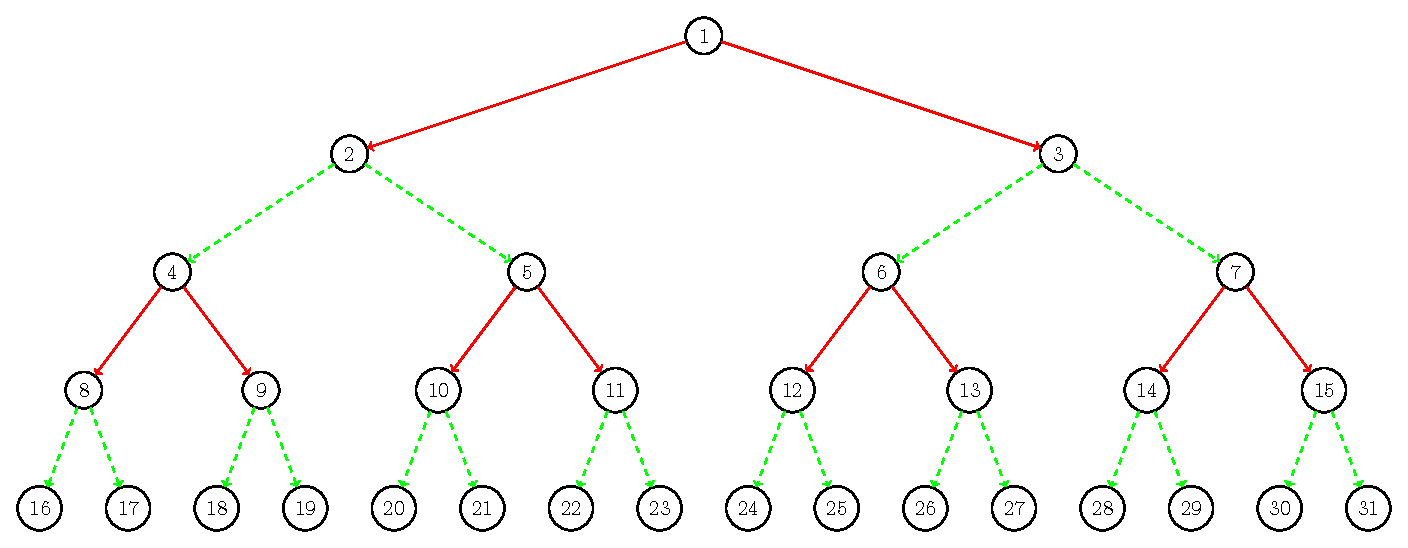
\includegraphics[width=.75\textwidth]{experiment1}
    \caption{Network structure (binary tree) for the first synthetic experiment. The active links of A(t) \chcomment{(use LaTeX)} alternate between the solid and dashed edges, with extra noise added at each time step, over a period of 10 cycles.}
    \label{fig:exp1}
    \bigskip
\end{figure}

Due to the hierarchy and timing of the edges, information appears to flow from lower indices to higher. The binary structure of the tree makes node 1 \chdeleted{to be} particularly efficient at transmitting information through the network, although this may not be immediately apparent in a single snapshot.

\chcomment{When referencing figures it is common to write 'Fig.' instead of 'Figure'.}

Figure \ref{fig:bt1} displays the dynamic broadcast centrality from Eq. \ref{eqn:u3.4}, at time $t=20$ for each of the 31 nodes. We observe that node 1 has a strong advantage in terms of centrality, and that centrality tends to decrease as the index increases. Nodes 2 and 5 are ranked higher than node 3, indicating that the additional noise has affected this part of the network. Since the maximum spectral radius of $\mathbf{A}(t)$ over the interval $[0, 20]$ is one \chcomment{(there is no way for the reader to see this)}, the parameter $\alpha=0.7$ was chosen with $\beta=0.1$, in this case. \chcomment{(Remind the reader what $\alpha$ and $\beta$ signifies.)}

Figure \ref{fig:bt2} depicts the same results with a lower $\beta=0.01$ value, which increases the contribution of older walks. As a reminder, if we consider a walk starting at time zero, then the  downweighting factor becomes $e^{−20 \times 0.01} \approx 0.8$ rather than $e^{−20 \times 0.1} \approx 0.1$. This change of the $\beta$ parameter has a negligible effect on the node rankings which makes sense considering that the network dynamics have an underlying periodic pattern, but it can be observed that it generates larger absolute values.

In Figure \ref{fig:bt3}, we return to the original $\beta=0.1$ value and set $\alpha$ to 0.1, resulting in less marked differences in the node rankings. Even though node 1 continues to be the most central, the differences are less pronounced as its capability to initiate numerous dynamic walks of length 4 to nodes at the bottom of the hierarchy has less influence or weight.

Figure \ref{fig:bt4} illustrates the aggregate degree of each node, that is, the sum of out degrees over time for each node. For nodes 1 to 15 in the binary tree structure, this value is 20, \chcomment{(How can I see this?)} which fluctuates due to the introduced noise. This graph highlights that the overall bandwidth \chcomment{(What does bandwidth mean in this context?)} can be a misleading network metric for determining node influence. \chcomment{(What choices of $\alpha$ and $\beta$ have you used in this experiment?)}

\begin{figure}[h]
     \centering
     \begin{subfigure}[b]{0.4\textwidth}
         \centering
         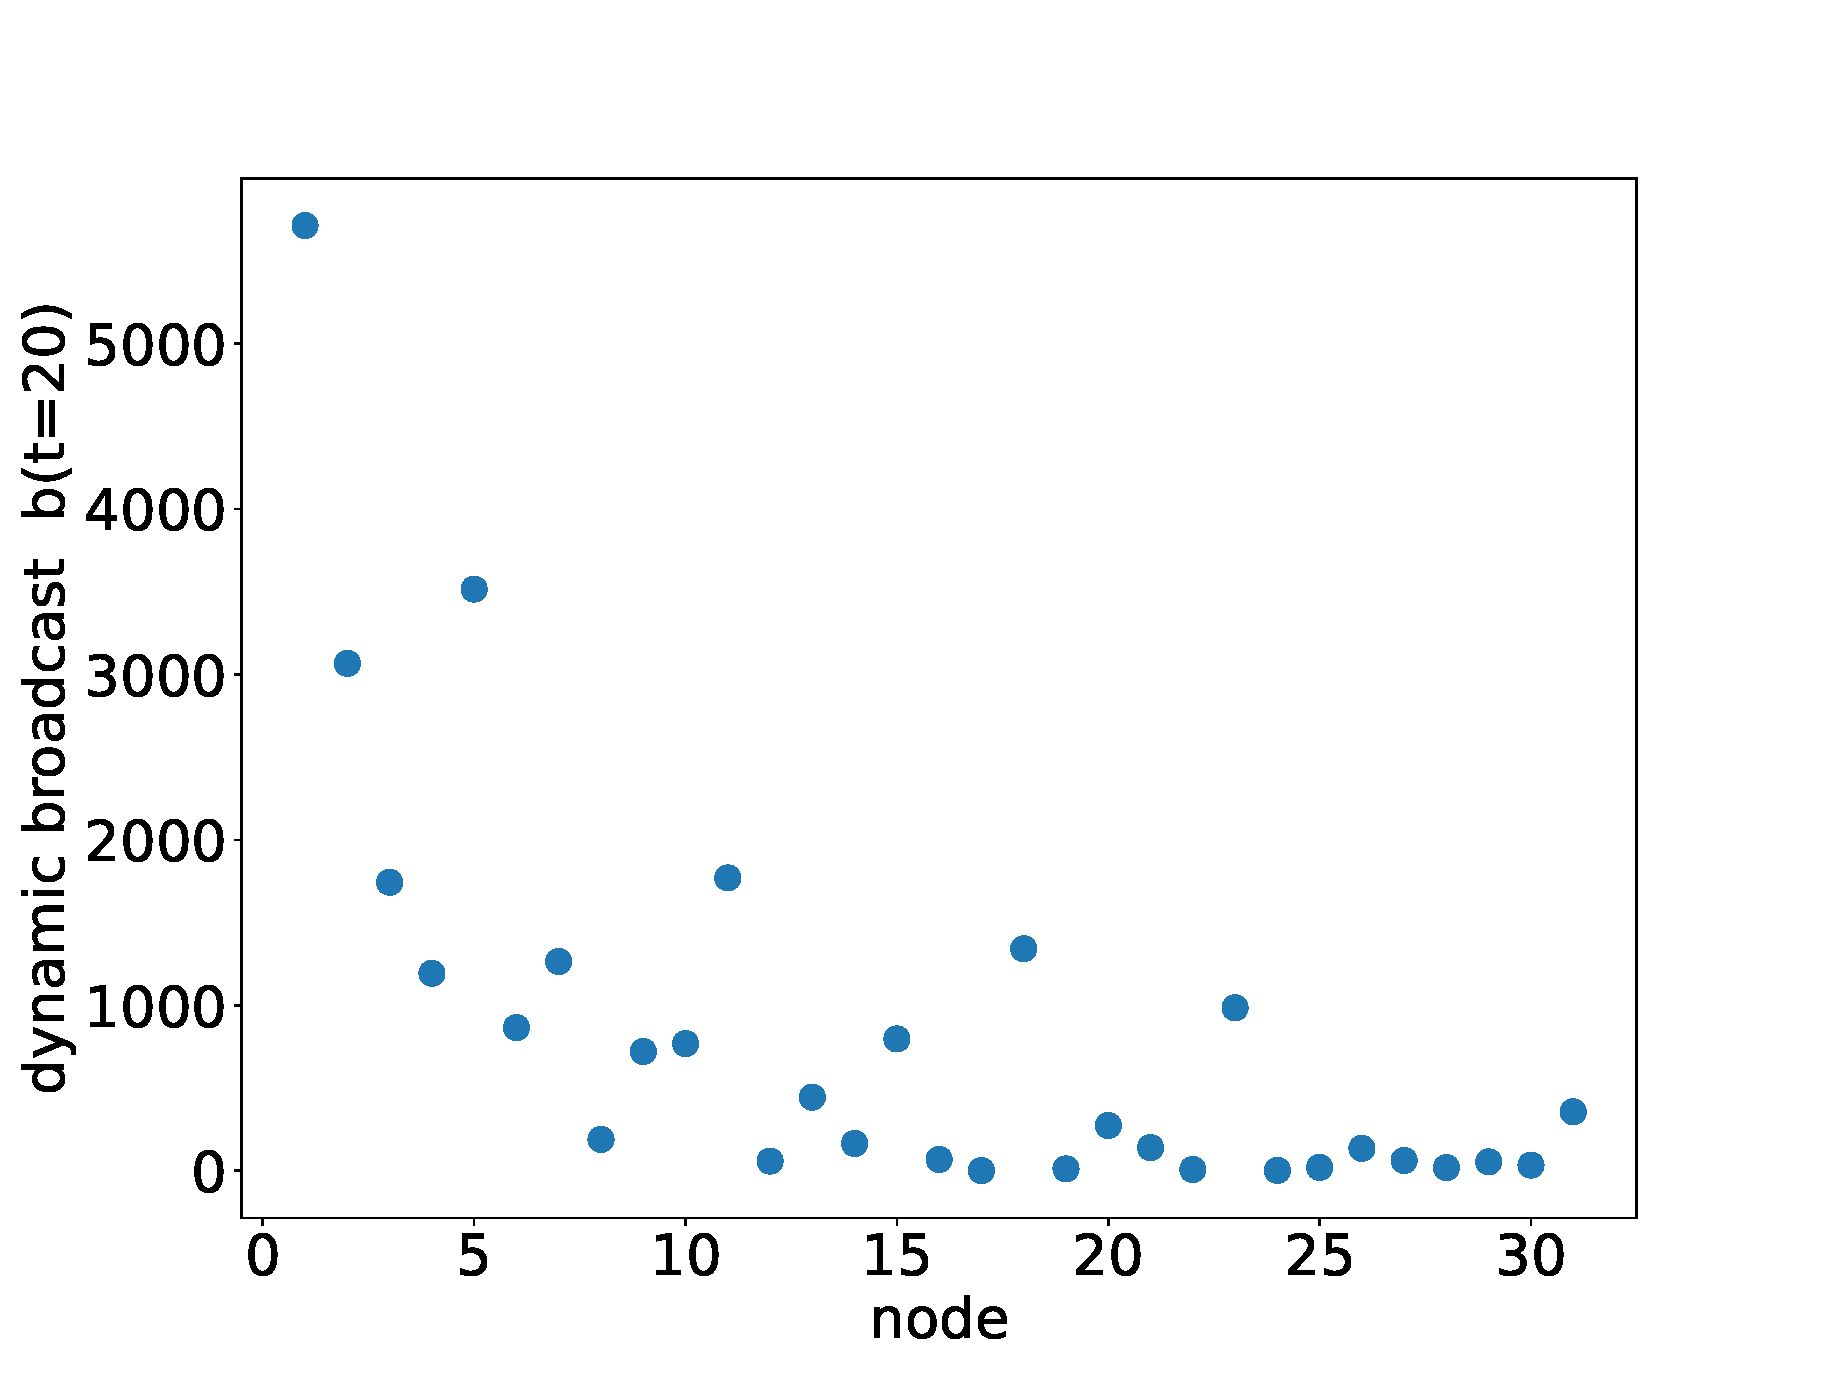
\includegraphics[width=\textwidth]{exp1_bt20a}
         \caption{Broadcast centrality for $\alpha = 0.7 ,~\beta = 0.1$}
         \label{fig:bt1}
     \end{subfigure}
     \hspace{0.5cm}
     \begin{subfigure}[b]{0.4\textwidth}
         \centering
         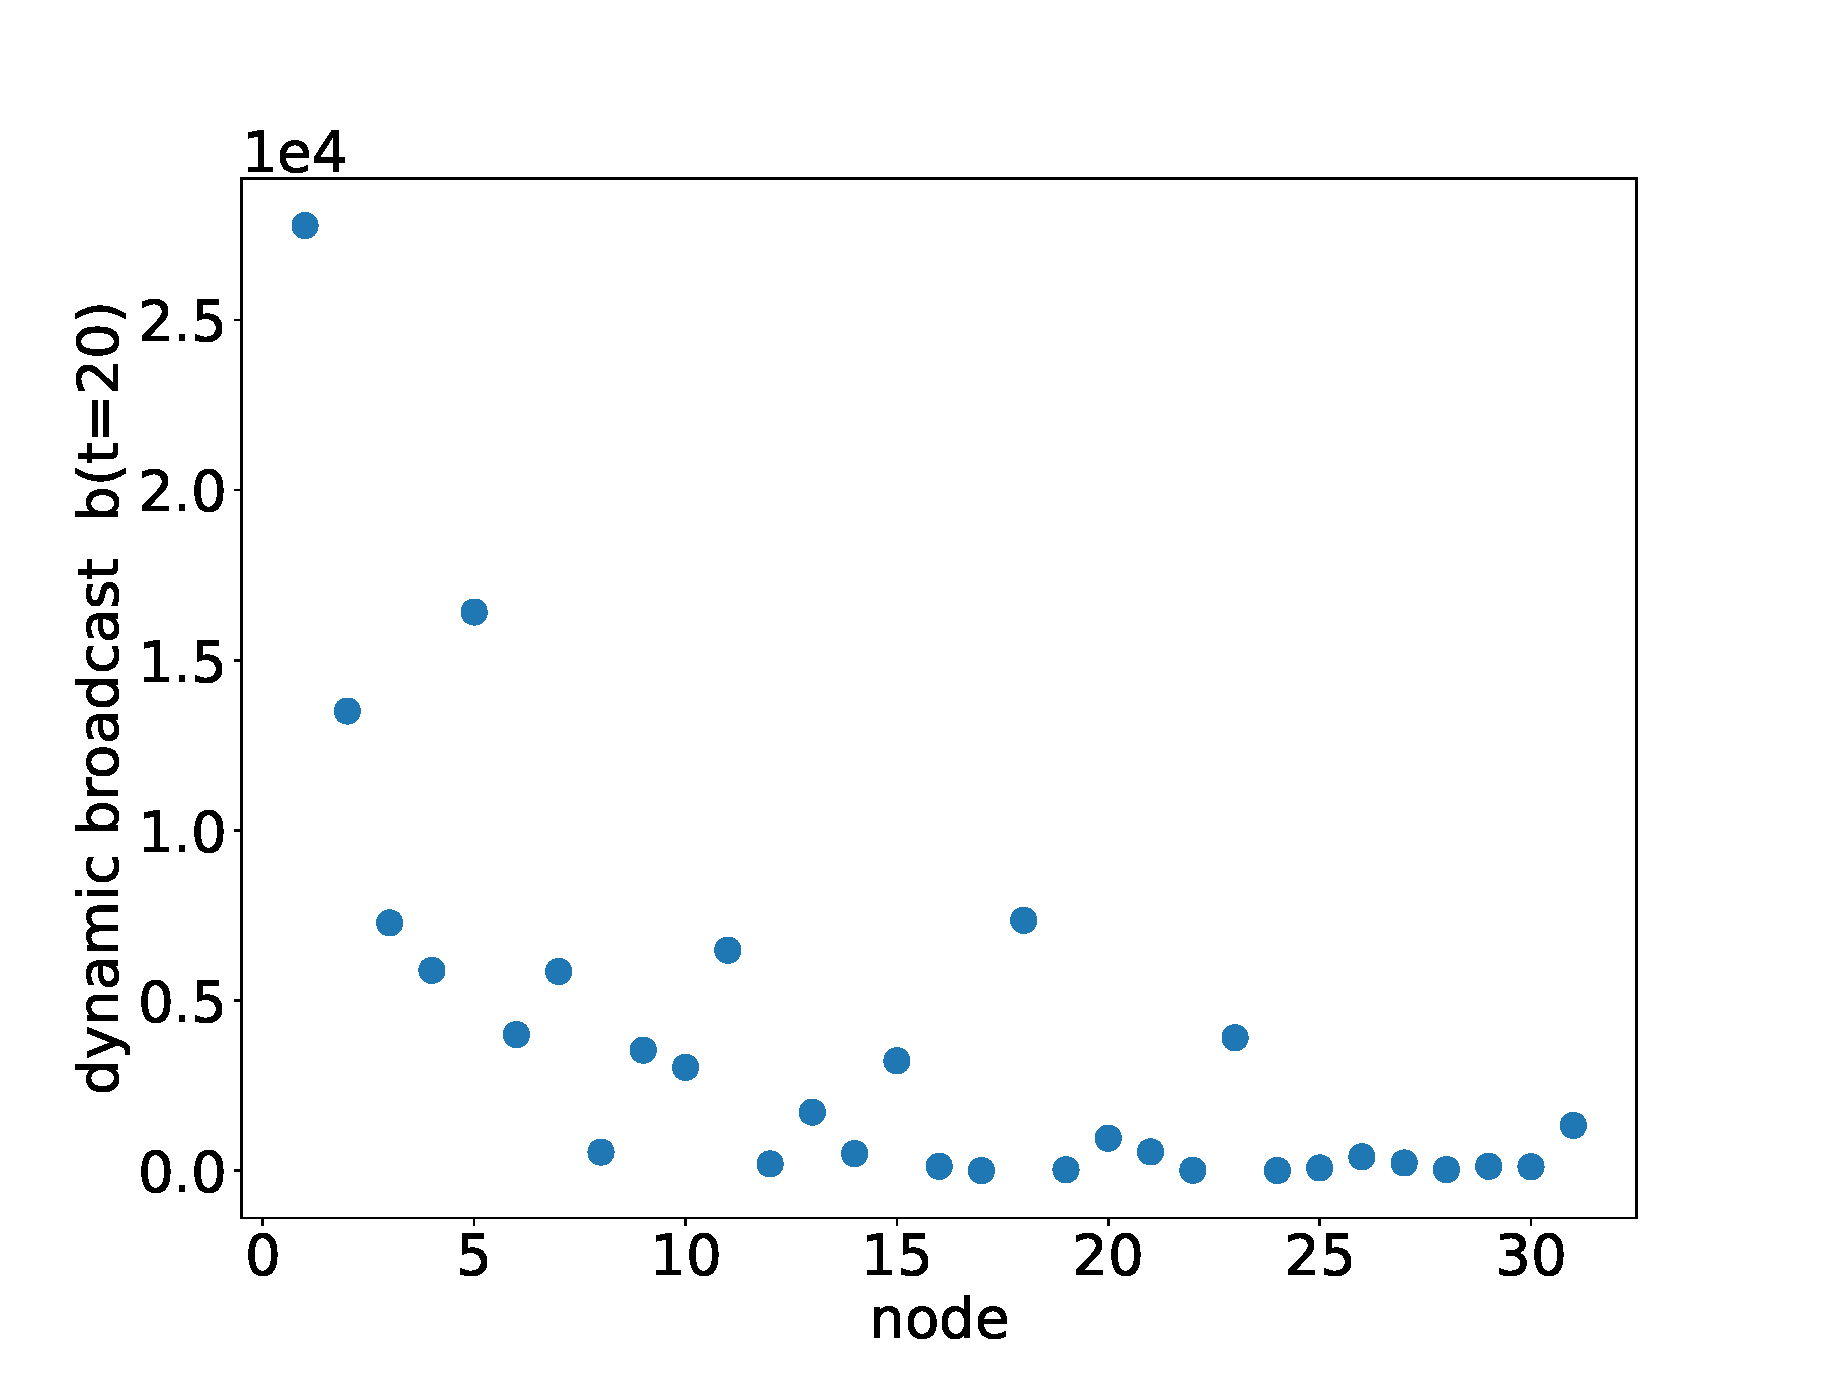
\includegraphics[width=\textwidth]{exp1_bt20b}
         \caption{Broadcast centrality for $\alpha = 0.7 ,~\beta = 0.01$}
         \label{fig:bt2}
     \end{subfigure}
     
     \begin{subfigure}[b]{0.4\textwidth}
         \centering
         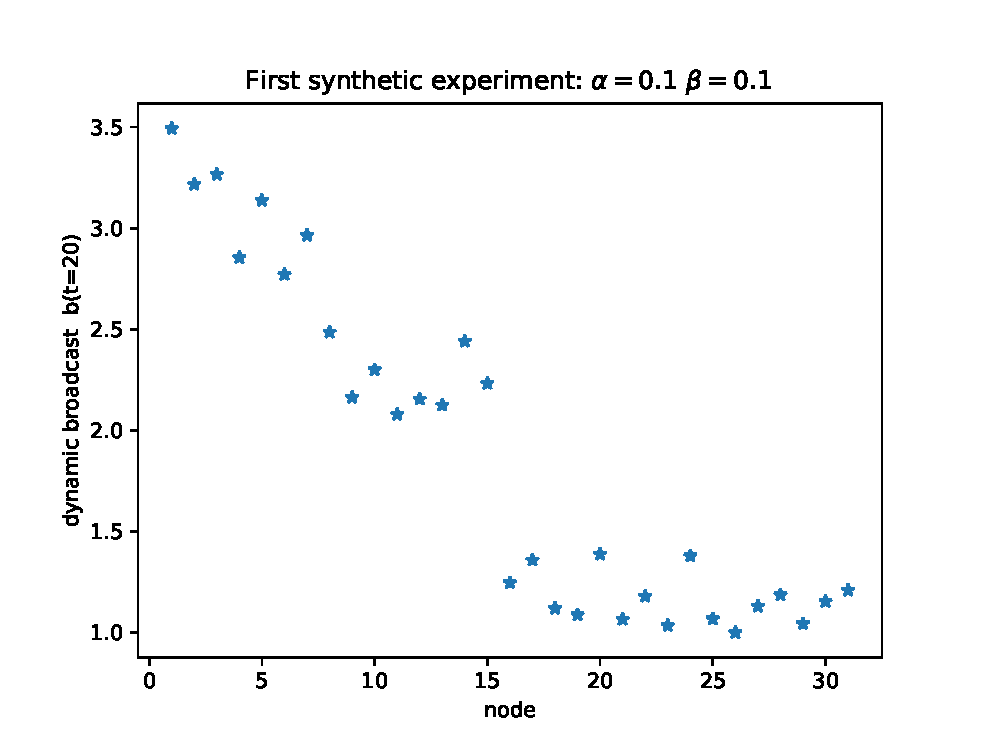
\includegraphics[width=\textwidth]{exp1_bt20c}
         \caption{Broadcast centrality for $\alpha = 0.1 ,~\beta = 0.1$}
         \label{fig:bt3}
     \end{subfigure}
     \hspace{0.5cm}
     \begin{subfigure}[b]{0.4\textwidth}
         \centering
         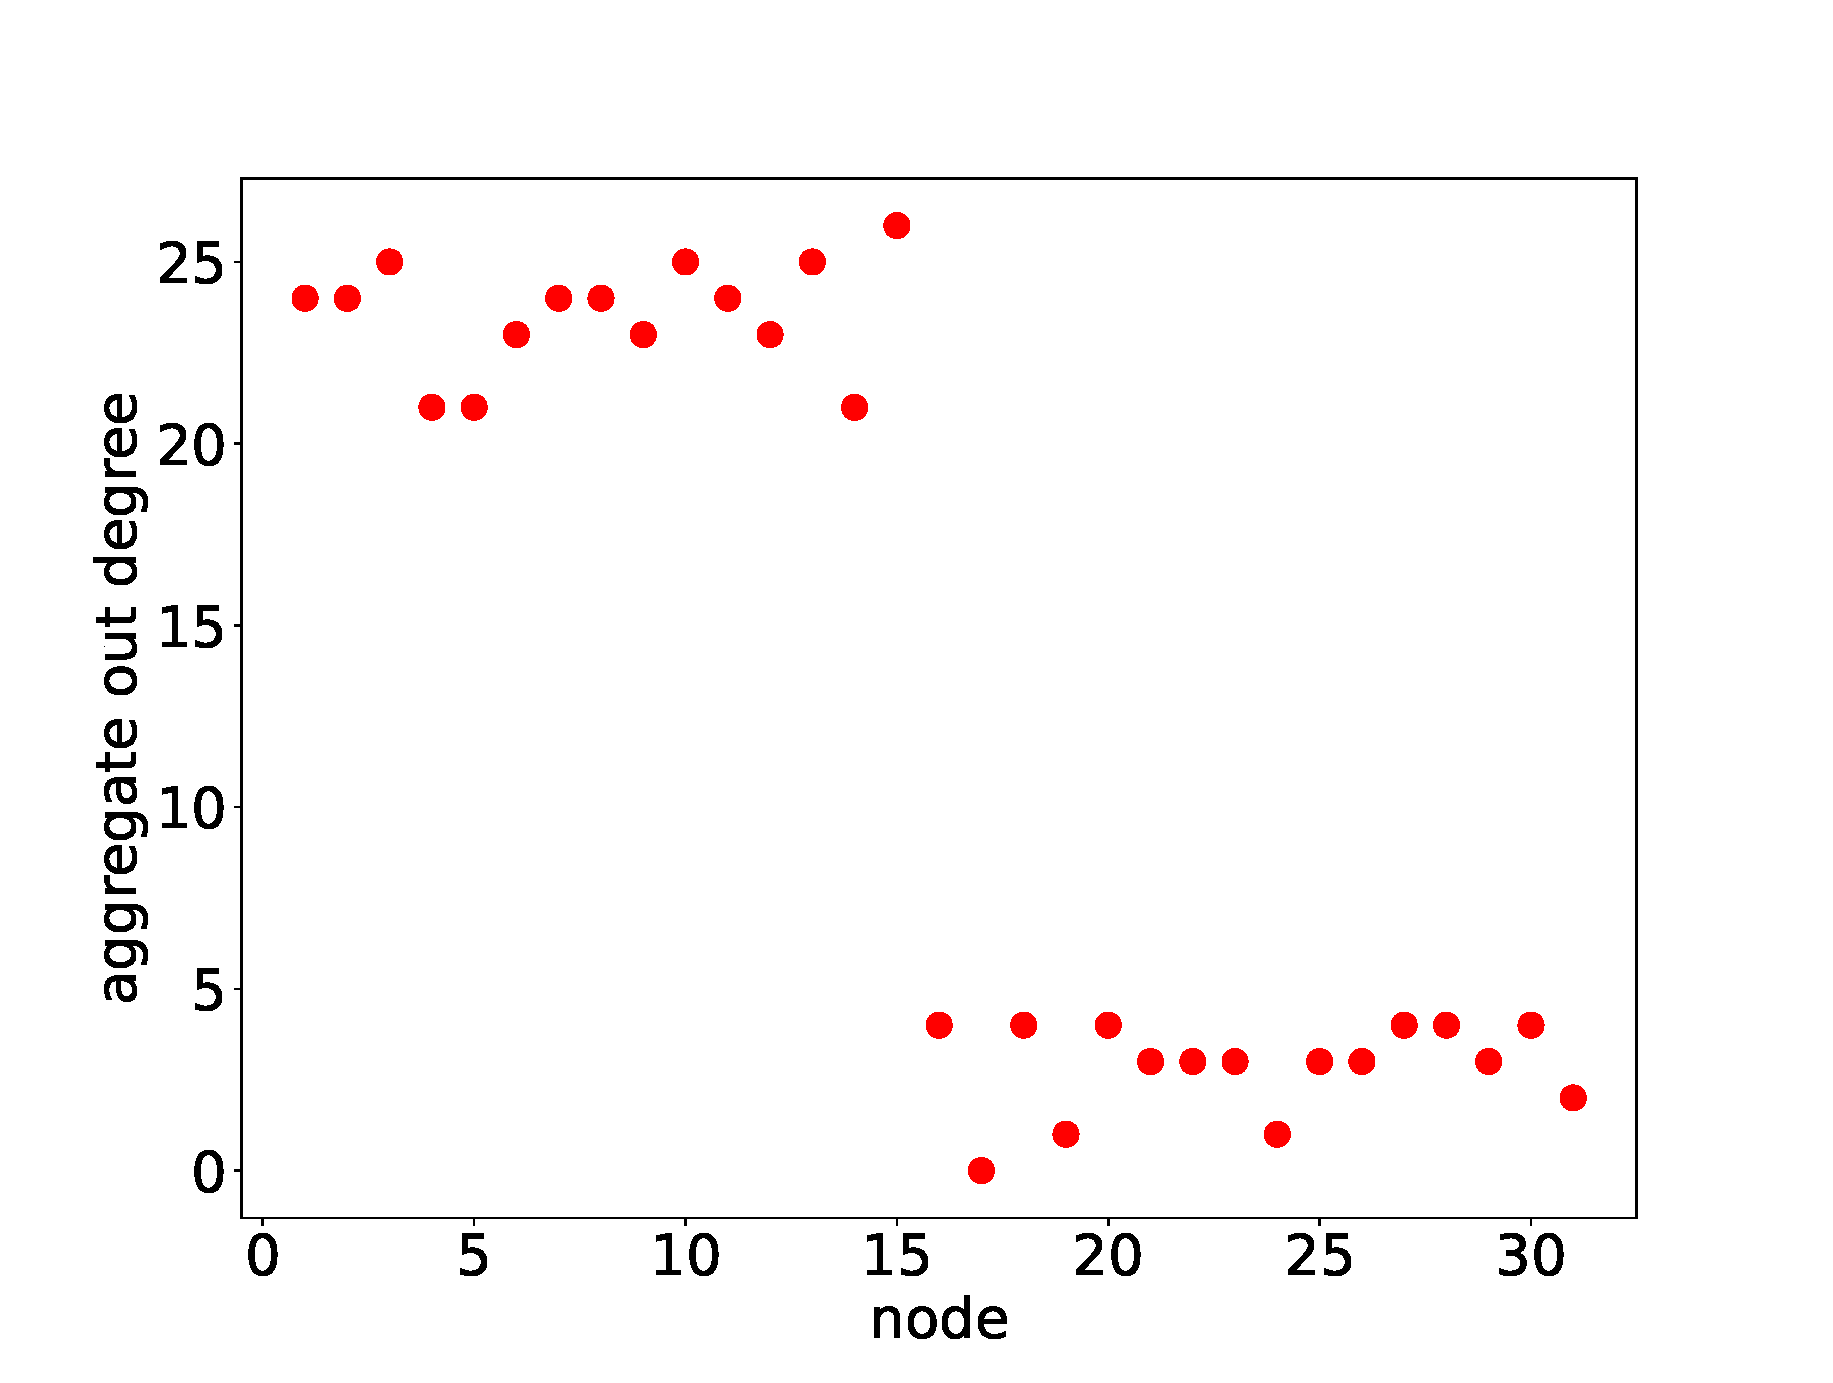
\includegraphics[width=\textwidth]{exp1_agg_out_degree}
         \caption{Aggregate out degree for each node}
         \label{fig:bt4}
     \end{subfigure}
        \caption{Results from the dynamic network in figure \ref{fig:exp1}.}
        \label{fig:fourbt}
\end{figure}

\chcomment{Make the title and figure labels larger.}

\chcomment{Summarize briefly what we have learnt from this experiment. Were the outcomes as expected? Any surprises?}

\newpage
\chcomment{I suggest that you make each experiment a separate subsection.}

\chcomment{What do we expect to learn from this experiment? In what way(s) is it different from the previous one?}

We now consider the second synthetic experiment from \cite{grindrod2014dynamical}. The experiment simulates multiple rounds of voice calls that occur along an undirected binary tree structure. Each node in the tree has at most one active edge at any given time, meaning that there are no "conference" calls.  Figure \ref{fig:exp2} shows the network with labels assigned to the edges indicating when they are active. 

The adjacency matrix, $\mathbf{A}(t)$, for this experiment is defined based on the ordered and non-overlapping time intervals such that $t_i\coloneqq[(i − 1)\tau , (i − 1 + 0.9)\tau )$, for $i=0, 1, \dots , 7$, and $\tau =0.1$.

\begin{figure}[h]\centering
    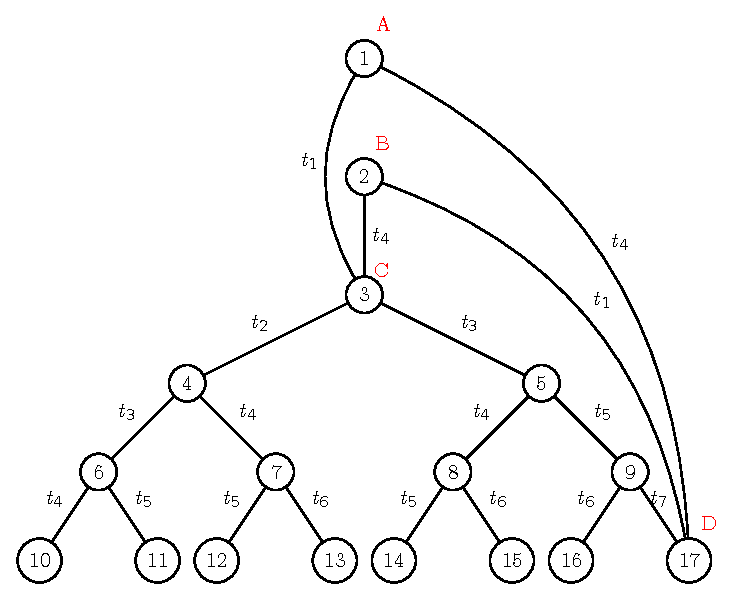
\includegraphics[width=.65\textwidth]{experiment2}
    \caption{Network structure for the second synthetic experiment. Links of A(t) \chcomment{(Use LaTeX)} are active over non-overlapping time intervals such that $t_i\coloneqq[(i − 1)\tau , (i − 1 + 0.9)\tau )$, for $i=0, 1, \dots , 7$, and $\tau =0.1$, repeated periodically over five cycles.}
    \label{fig:exp2}
    \bigskip
\end{figure}

The dynamic network is constructed in a way that node A is designed to be a more effective influencer compared to node B. This can be attributed to several factors such as a higher social/business status or access to more current and relevant information. Connections are built in such a way that node A talks to node C in $t_1$, initiating the cascade of phone calls in the network. On the other hand, node B waits until $t_4$ to contact node C, which does not trigger any new cascades. In this scenario, all the adjacency matrices for each time interval turn out to have unitary spectral radius.

\chcomment{What does $\mathbf{A}(t)$ look like? What are the value of the nodes? How many nodes are there? Is it symmetric? Are the eigenvalues real? Keep the reader informed so that the experiment can be reproduced.}

The experiment is repeated over five cycles, during which nodes A and B send out a total of 10 messages. Even if nodes A and B have an apparent identical behaviour \chdeleted{from an overall perspective}, both contacting nodes C and D for the same length of time, the results in Figure \ref{fig:twobt} (for $\alpha = 0.7, \beta = 0.1$ and $\alpha = 0.9 , \beta = 0.1$ respectively) show that the dynamic broadcast centrality measure is able to capture the knock-on effect \chcomment{(What does 'knock-on effect' mean?)} enjoyed by node A (solid line) with respect to node B (dashed line). This difference in broadcast centrality is much more pronounced for values of $\alpha$ close to one (Figure \ref{fig:bt6}), where longer walks are more strongly penalized.

\begin{figure}
     \centering
     \begin{subfigure}[b]{0.49\textwidth}
         \centering
         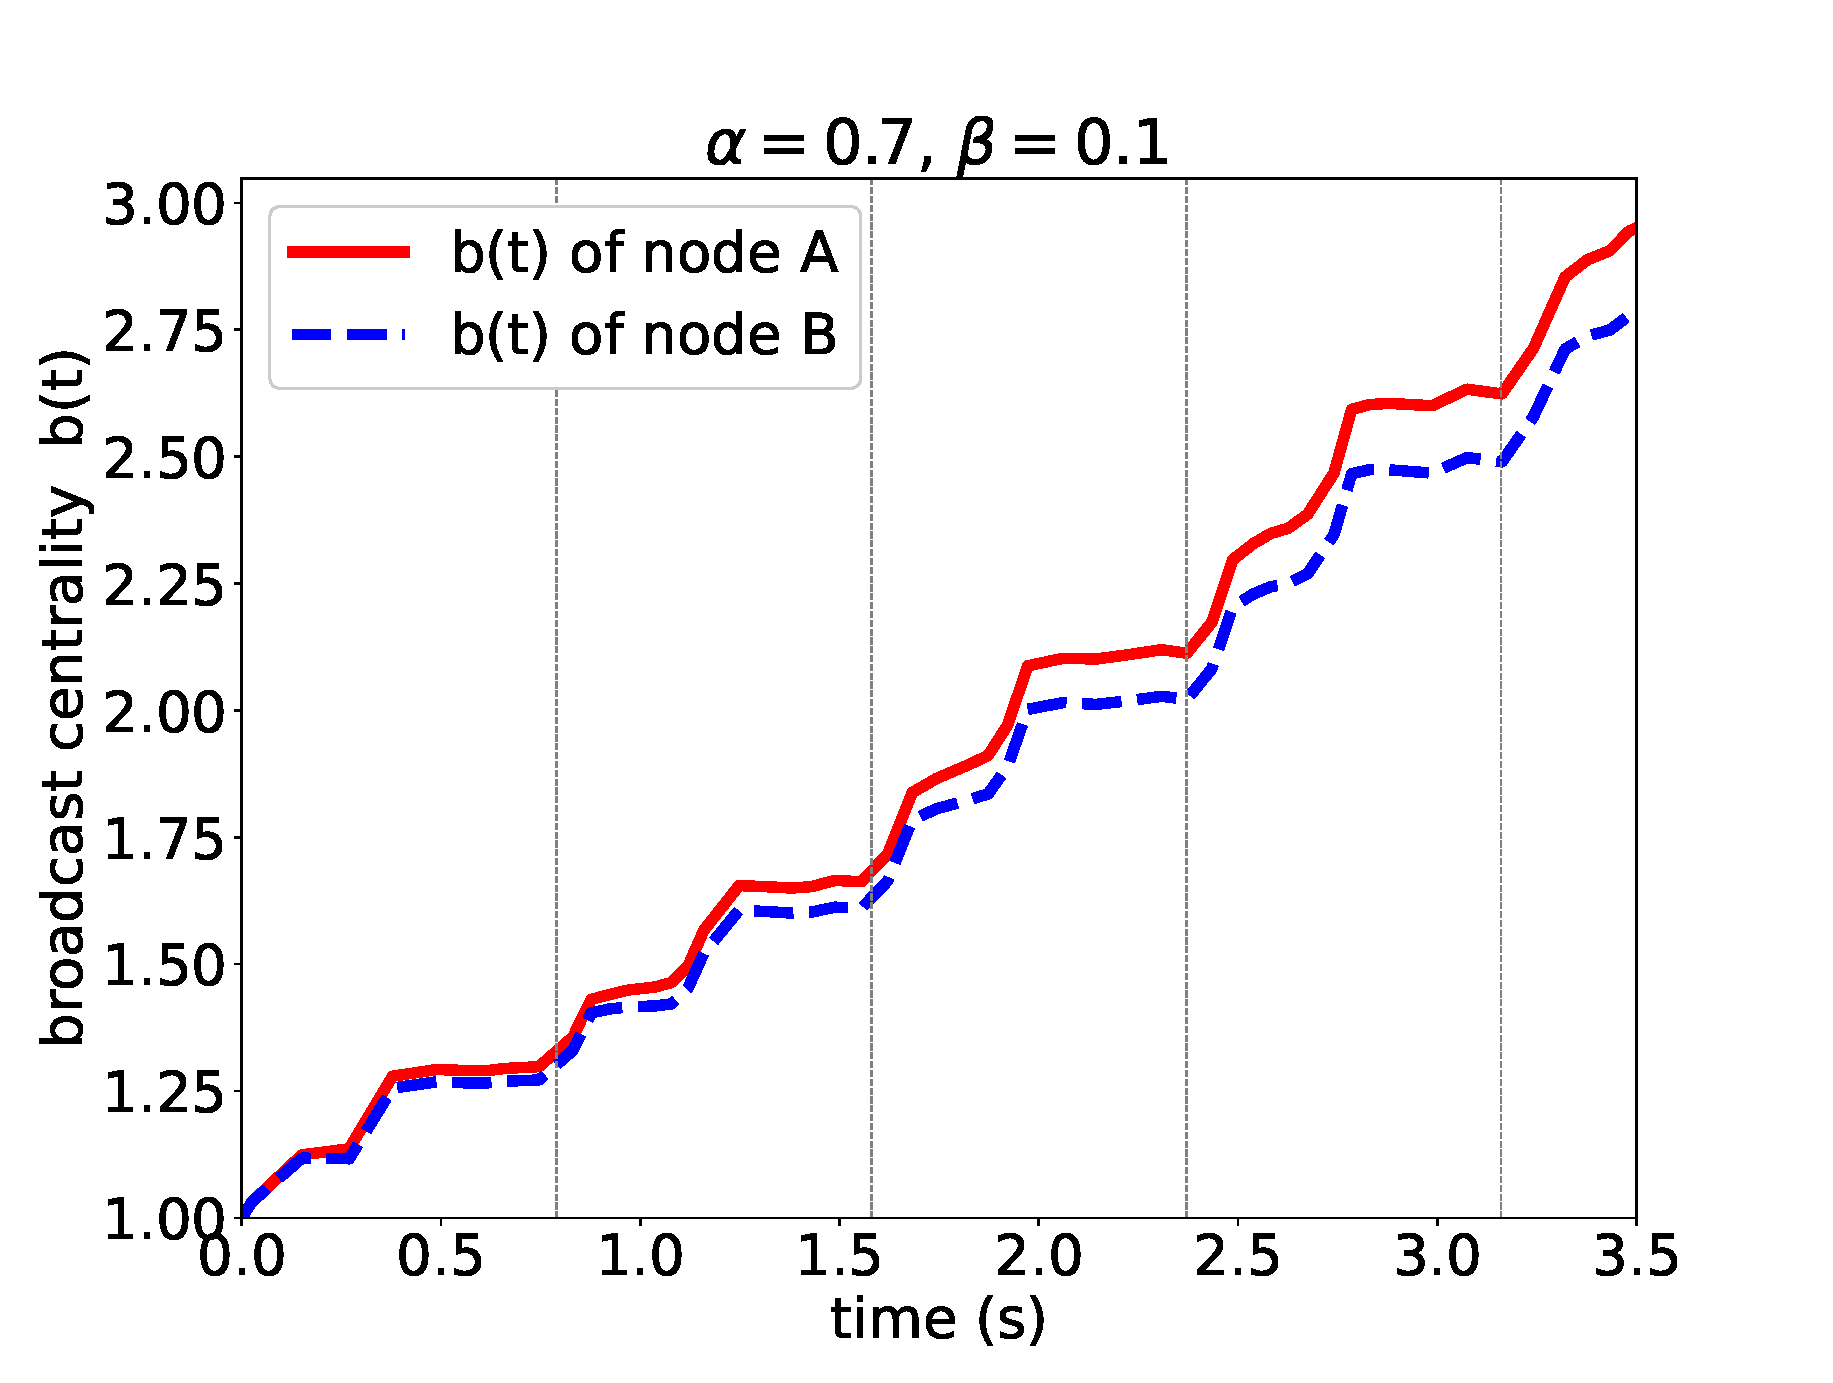
\includegraphics[width=\textwidth]{exp2b_btA_vs_btB}
         \caption{broadcast for $\alpha = 0.7 ,~\beta = 0.1$}
         \label{fig:bt5}
     \end{subfigure}
     \hfill
     \begin{subfigure}[b]{0.49\textwidth}
         \centering
         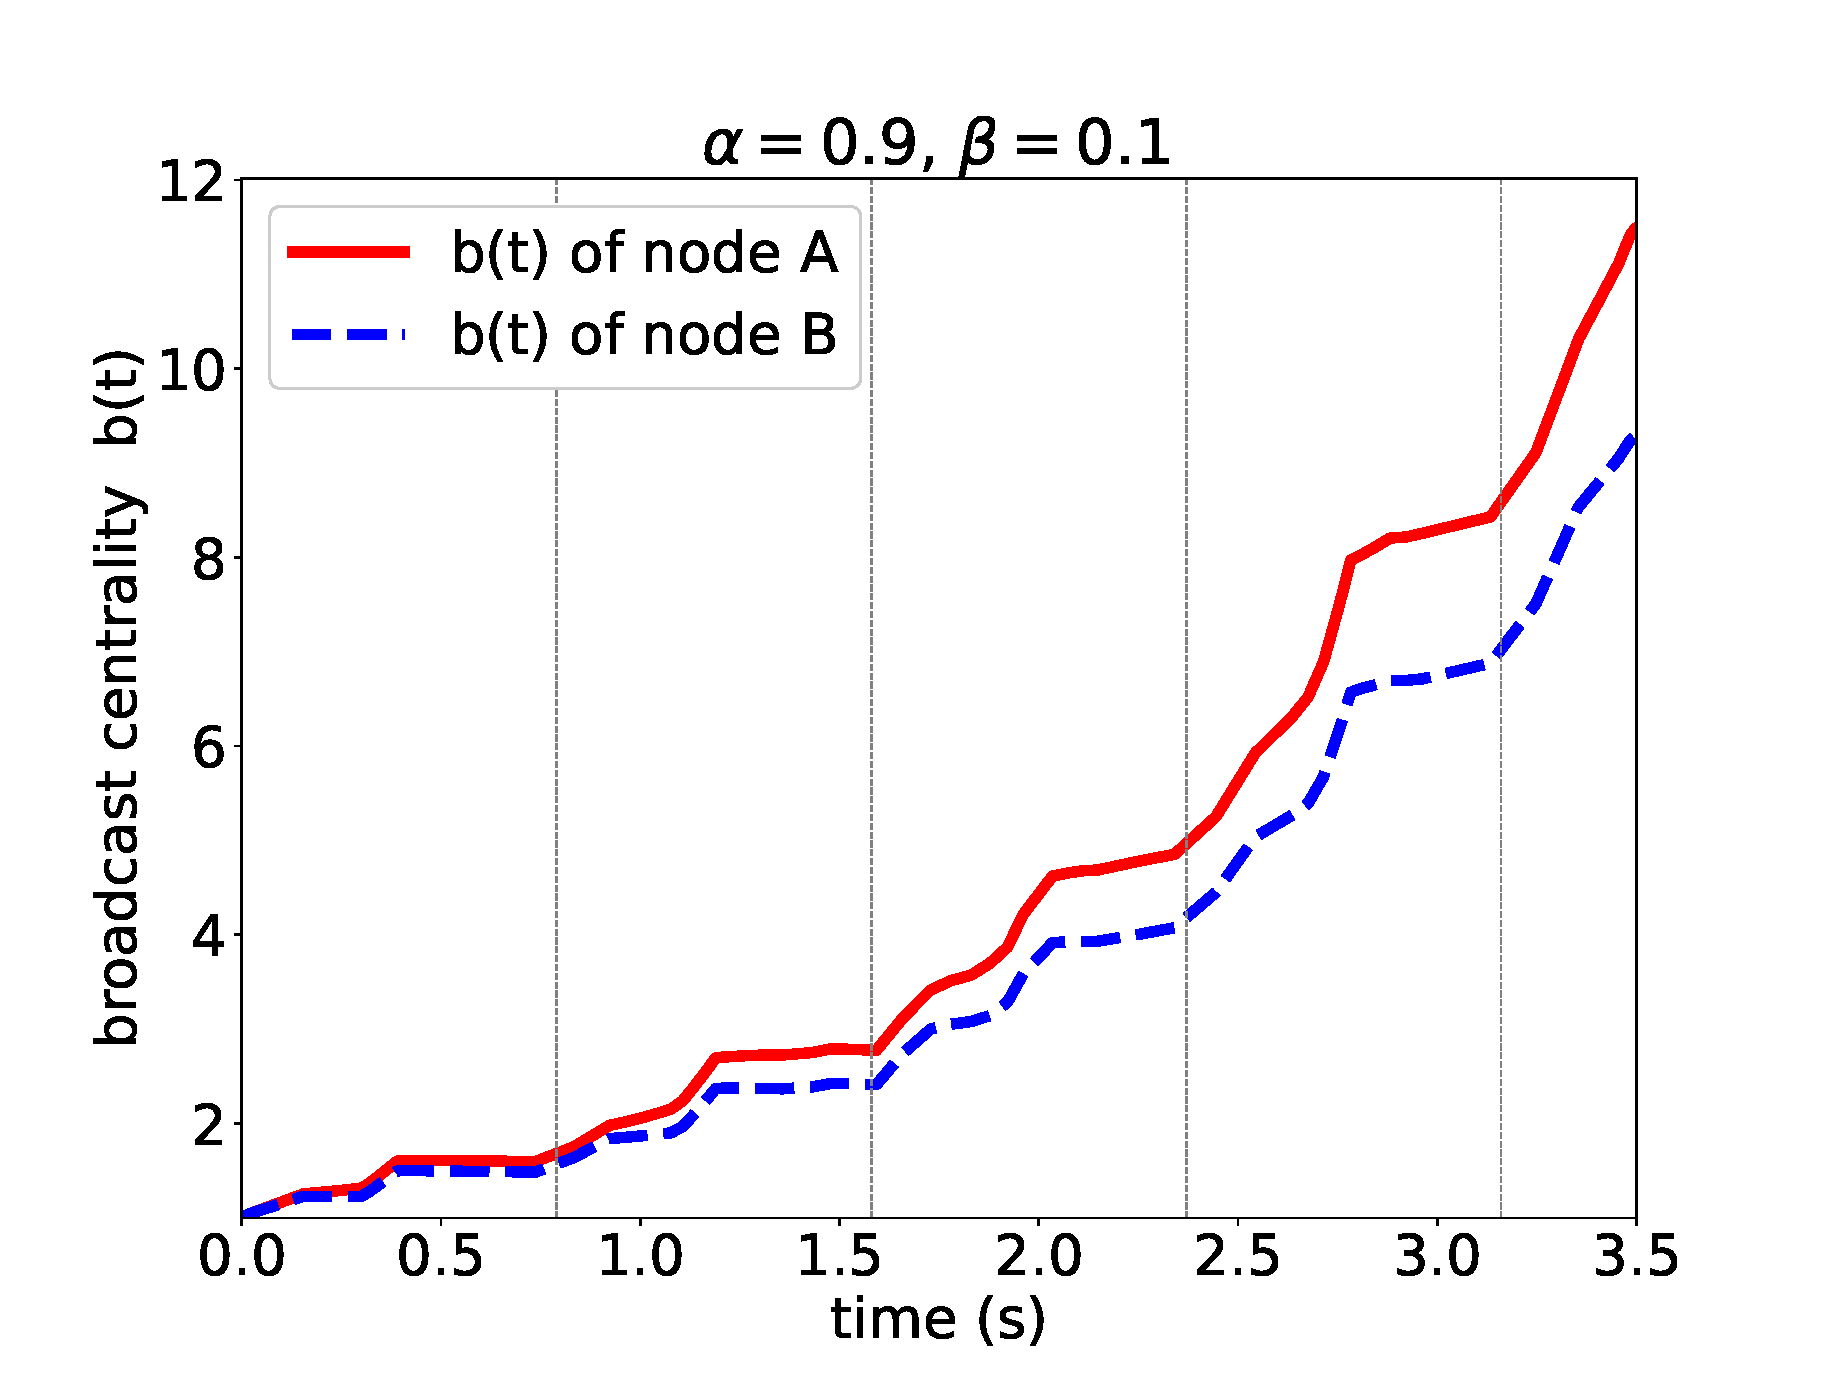
\includegraphics[width=\textwidth]{exp2a_btA_vs_btB}
         \caption{broadcast for $\alpha = 0.9 ,~\beta = 0.1$}
         \label{fig:bt6}
     \end{subfigure}
     \caption{Dynamic broadcast centrality over time for node A (solid) and node B (dashed) in the network of figure \ref{fig:exp2}.}
     \label{fig:twobt}
\end{figure}

\chcomment{Make titles, axis lables and legends larger in all Figures.}

\chcomment{Try to explain with a few words why the broadcast centrality looks the way it does, i.e. why is it increasing and why does it look like a series of steps?}

\chcomment{Out of curiosity, do you know what the broadcast centrality looks like for the other nodes? Anything interesting to discuss there?}

\section{Voice call experiment}
\label{sec:voicecall}
The next experiment applies the new modelling framework (Eq. \ref{eqn:u3.3}) to a set of voice call interactions, in order to analyze the dynamic behavior of a fictitious, controversial socio-political movement. The data used for the experiment, supplied as part of the IEEE VAST 2008 Challenge \cite{grinstein2008vast}, consists of a complete set of 9834 time-stamped calls across 400 cell phone users over a 10 day period, with information on IDs for the send and receive nodes, start time in hours/minutes, and duration in seconds.

The aim of the experiment is to show the usefulness of the new matrix ODE in dealing with this type of dynamic network, comparing dynamical measures against aggregated. To that end, the bandwidth of a node is defined as the aggregate number of seconds for which the node ID is active as a sender or receiver. This will allow us to compare the effective activation time of a certain node with its relevance in terms of dynamic broadcast centrality.

\chcomment{The above paragraph is very good! It explains the goals, what will be done and defines special terms necessary to understand the particular experiment. Try to emulate this paragraph at the start of the previous two experiments.}

The designers of the above mentioned competition provided additional information indicating that node 200 was the leader of an important community who controlled a closely connected subnetwork or inner circle consisting of nodes 1, 2, 3, and 5. However, starting from day 7, these individuals seem to have switched their phone IDs: node 200 became 300, and the others became 306, 309, 360, and 392.

For this experiment, $\mathbf{A}(t)$ was assumed to be symmetric, meaning that $\mathbf{A}_{ij}(t) = \mathbf{A}_{ji}(t) = 1$ if nodes $i$ and $j$ were communicating at time $t$, which was measured in seconds. Parameters $\beta$ was chosen to be approximately $\beta = 1/(60\times 60 \times 24) \approx 1.2 \times 10^{-5}$, which corresponded to a time downweighting of $e^{-1}$ per day, and set the edge attenuation parameter $\alpha$ to a similar value of $10^{-4}$. The SciPy's \texttt{solve\_ivp} method was used to numerically solve the ODE (\ref{eqn:u3.3}), which discretizes the time interval in an efficient and transparent way under the hood. Additionally, absolute and relative error tolerances were both set to $10^{-4}$. To improve efficiency, the matrix logarithm was approximated in this occasion with its expansion to the fifth power:

$$\log(\mathbf{I} - \alpha \mathbf{A}(t)) \approx \alpha \mathbf{A}(t) - \alpha^2 \mathbf{A}(t)^2/2 + \alpha^3 \mathbf{A}(t)^3/3 - \alpha^4 \mathbf{A}(t)^4/4 + \alpha^5 \mathbf{A}(t)^5/5$$ 

Visually speaking, the effects of increasing the number of terms in the expansion to 6 and 7 remained identical.

\chcomment{Again, very good description of the experiment!}

\chcomment{Is there are reason for changing from present tense to past tense in this section?}

This experiment yields two key findings:
\begin{enumerate}[label=(\roman*)]
  \item The dynamic broadcast/receive measures (Eqs. \ref{eqn:u3.4}) identified key nodes as highly influential, even if they were not actively using much bandwidth, without any prior knowledge of an inner circle's existence.
  \item The transformation \chadded{that} occurred in the network on day 7 was shown by the running centrality measures once we knew the IDs of the inner circle.
\end{enumerate}

\chcomment{To me it makes more sense to show the data first and draw the conclusions afterwards.}

\newpage

Figure \ref{fig:ve1a} was used to demonstrate point (i) by plotting bandwidth against dynamic broadcast, $\mathbf{b}(t)$, using data up until the end of day 6. Dynamic receive centrality, $\mathbf{r}(t)$, was also computed using its own vector-valued ODE (Eq. \ref{eqn:u4.1}) obtaining similar results and a computation time reduction of approximately $30\%$.

\chcomment{Show these results! Also describe how you measured the exection times of the two experiments. Make a table and refer to it when you claim that the computation is 30\% faster.}

The scatter plot also includes symbols to mark certain nodes, such as a downward pointing triangle for the ring leader, 200, and squares for the related inner-circle nodes, 1, 2, 3, and 5. The follow-on ID for the ringleader, 300, is marked with an upward pointing triangle, and those for other members, 306, 309, 360, and 392, are marked with diamonds.

The results showed that the key nodes for days 1-6 were much more dominant in terms of dynamic broadcast than overall bandwidth. Specifically, the ringleader node had a low bandwidth but ranked sixth out of 400 in terms of broadcast communicability.

\begin{figure}[h]
     \centering
     \begin{subfigure}[b]{0.49\textwidth}
         \centering
         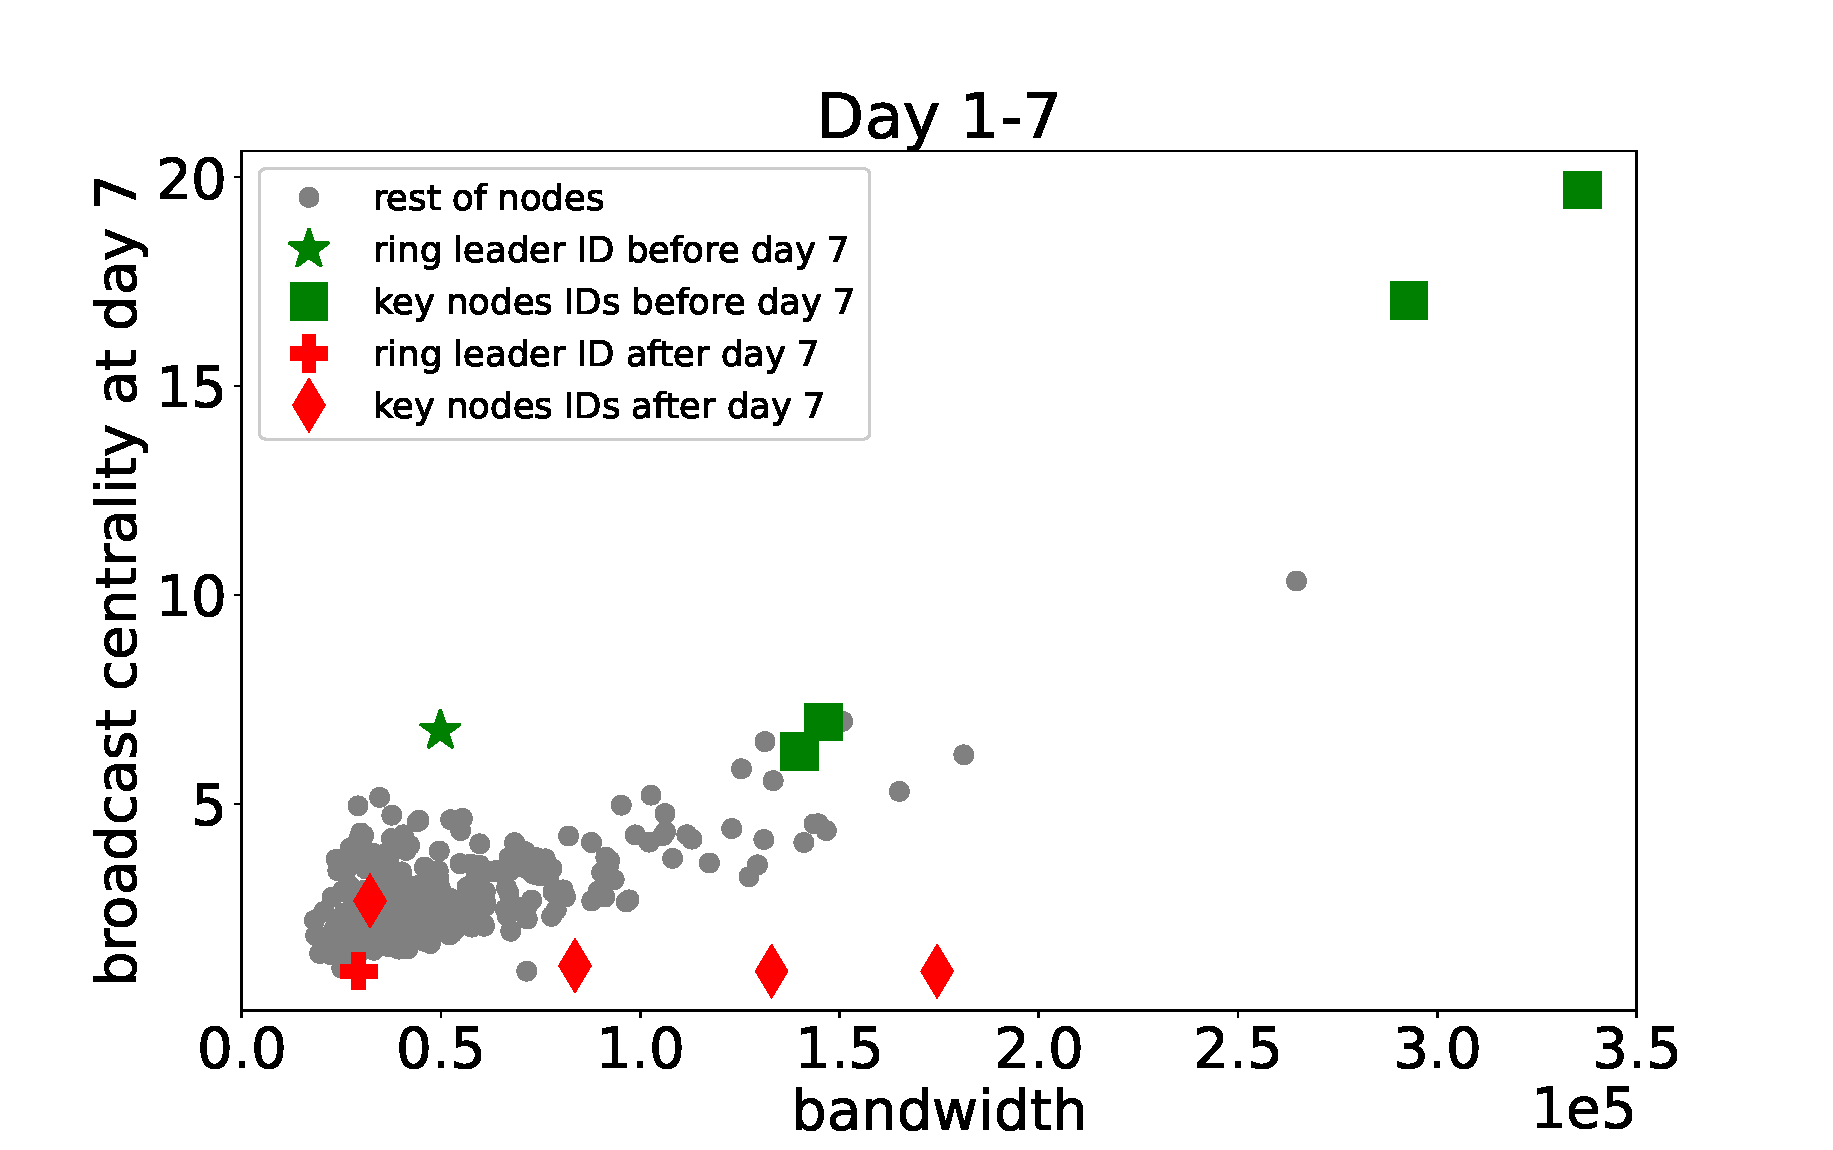
\includegraphics[width=\textwidth]{voicecall_exp_1_7}
         \caption{broadcast centrality at the end of day 6 vs. bandwidth (secs.)}
         \label{fig:ve1a}
     \end{subfigure}
     \hfill
     \begin{subfigure}[b]{0.49\textwidth}
         \centering
         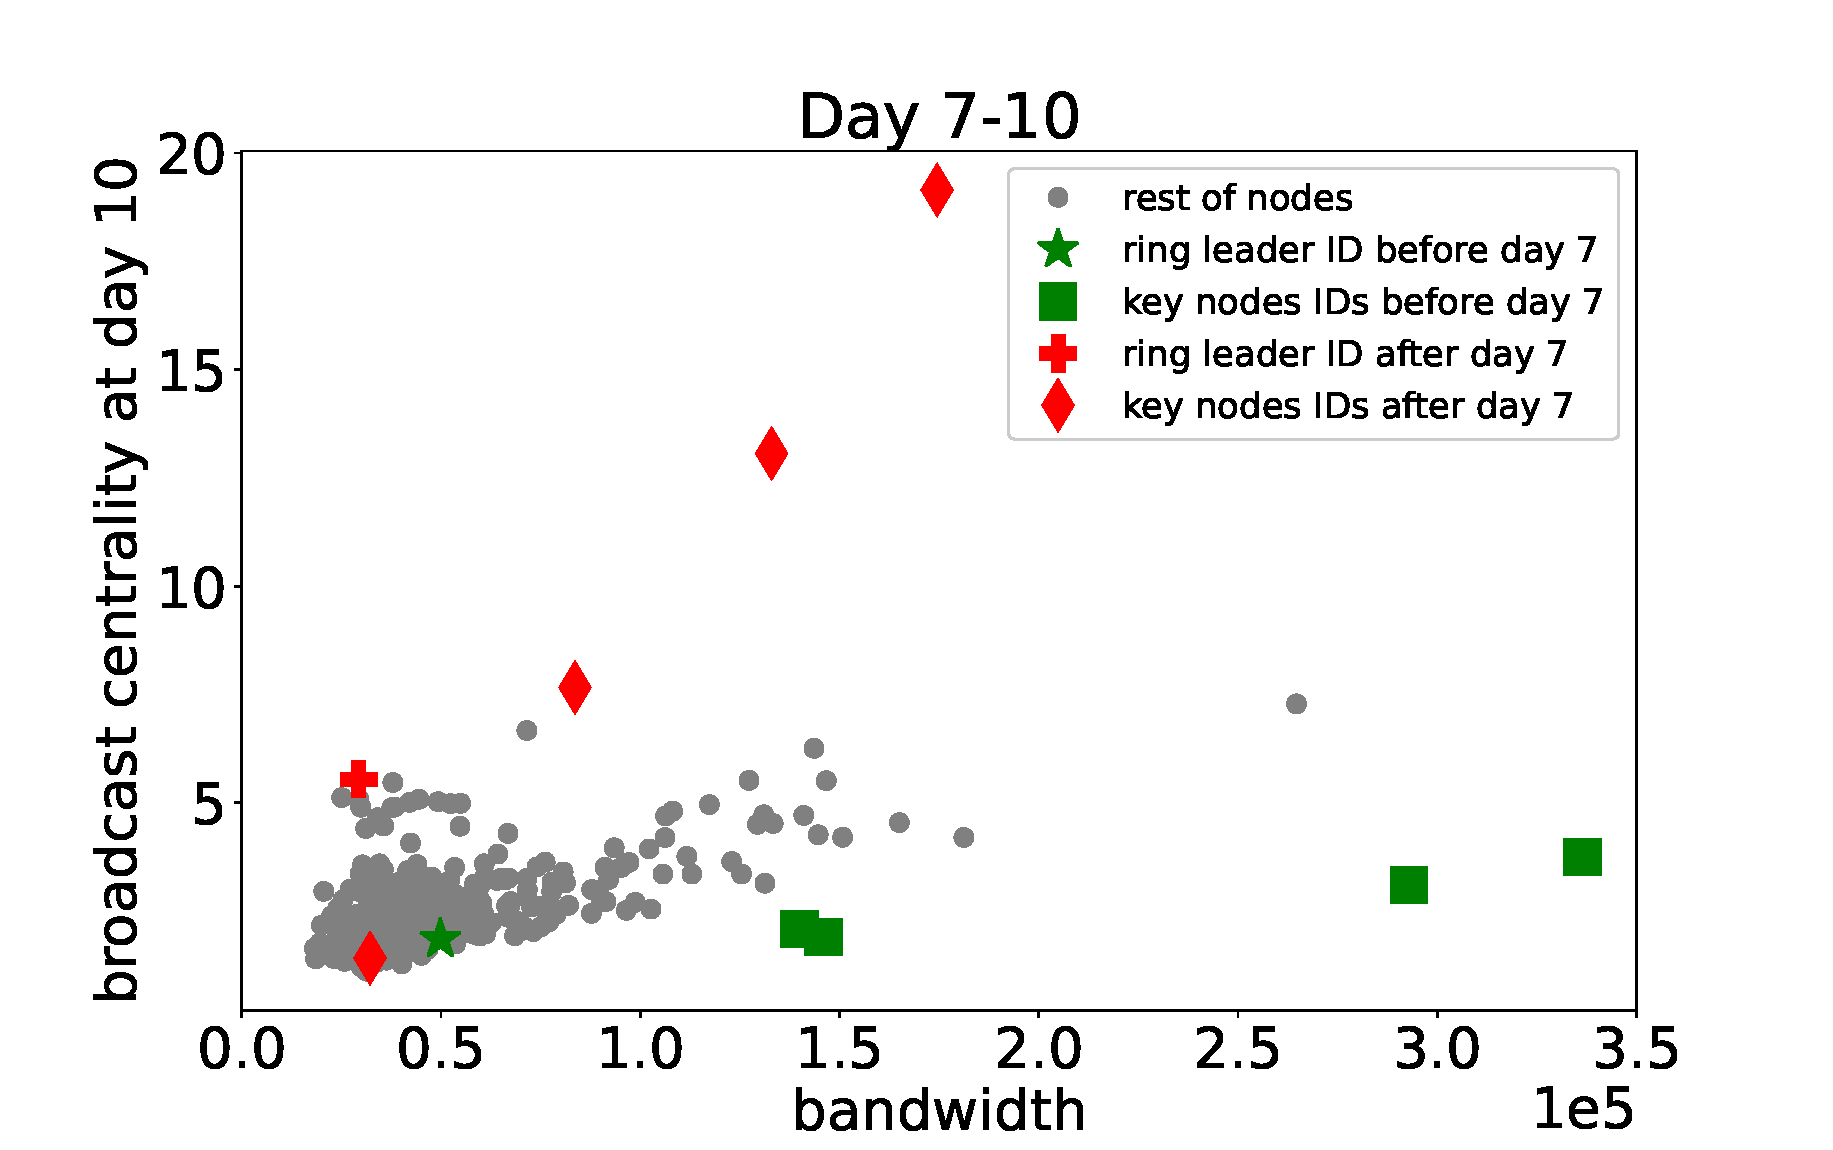
\includegraphics[width=\textwidth]{voicecall_exp_7_10}
         \caption{broadcast centrality at the end of day 10 vs. bandwidth (secs.)}
         \label{fig:ve1b}
     \end{subfigure}
     \caption{Dynamic broadcast measure for each node vs. node's bandwidth from voice call data.}
     \label{fig:ve1}
\end{figure}

\chcomment{Bigger Figures! It is very hard to see anything at the moment.}

The data from days 7 to 10 is displayed in Figure \ref{fig:ve1b}, and it confirms that the dynamic broadcast score is a more effective indicator of centrality than overall bandwidth in uncovering the inner circle. \chcomment{(I would move the previous conclusion to the end of the paragraph.)} The plot shows how the new ID of the ringleader, that is indicated with an upward pointing triangle, has a low overall bandwidth, but ranks seventh highest for broadcast centrality. Although the former IDs from the inner circle, marked with squares, still possess high bandwidth, their low dynamic broadcast scores suggest that they are no longer central players.

\chcomment{Very good description of the data. It tells the reader exactly how to interpret the results and what we have learnt.}

\newpage

The communicability between the original IDs of the five most important players (ID nodes: 200, 1, 2, 3, and 5) is presented in Figure \ref{fig:ve2} to support point (ii). The graph shows how communication between these key nodes changes over a ten days period of time. At each discretized time point, the average amount of messages, broadcast ($U_{ij}$) and received ($U_{ji}$), between each pair of key nodes is measured and then scaled by the average amount of communication between all pairs of nodes in the network. By analyzing this measure, we can observe how the network changes over time, especially when the players start using different IDs after day 7.

\chcomment{In this section you use the concept of comminucability first, and define it later. Do it the other way around. Also, you can quite easily express the definitio in mathematical terms rather than in text.}

\begin{figure}[h]\centering
    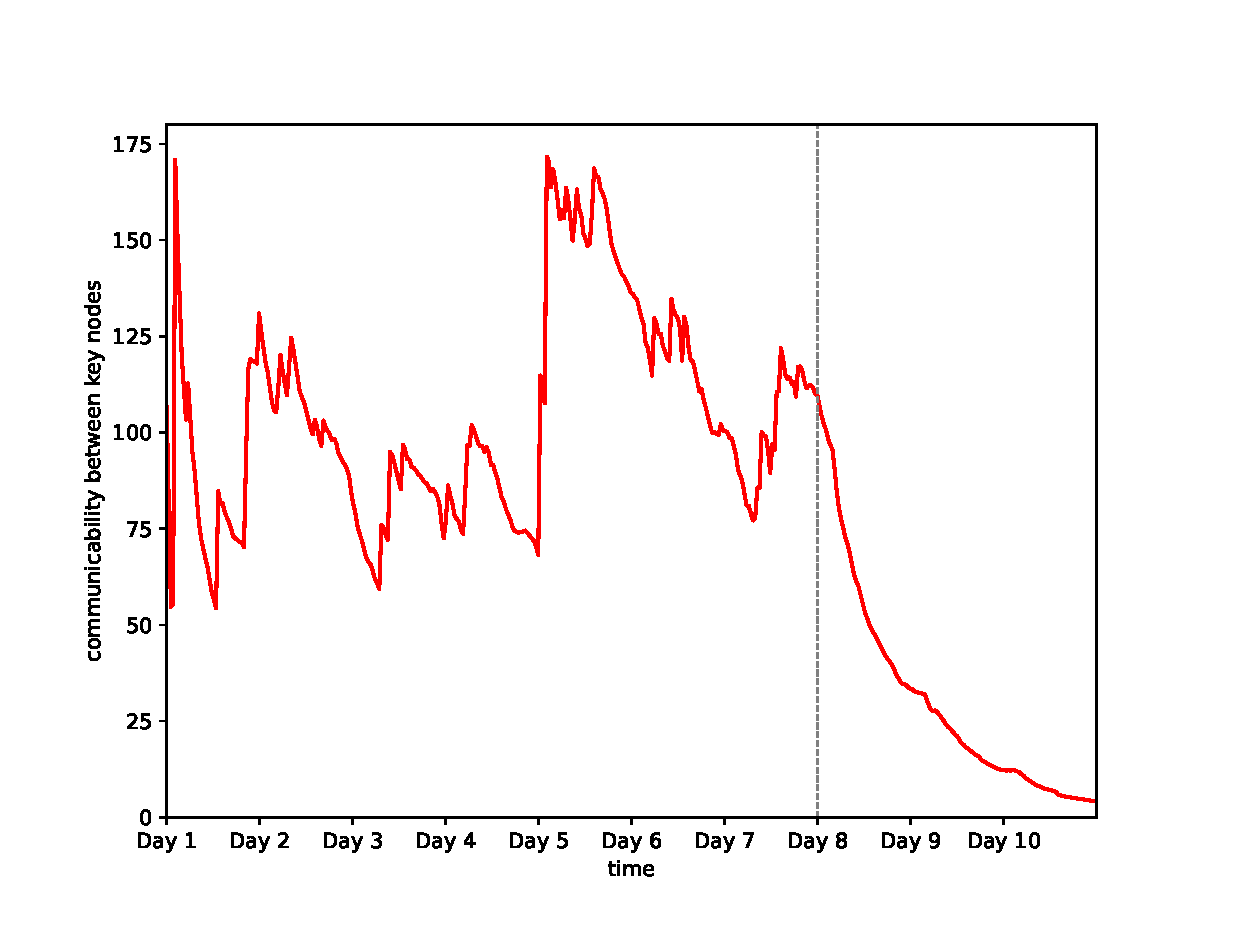
\includegraphics[width=.79\textwidth]{voicecall_exp_dyncomm}
    \caption{Voice call data: dynamic communicability between the five key nodes as a function of time.}
    \label{fig:ve2}
    \bigskip
\end{figure}

\chcomment{Make the axis labels larger.}

\chcomment{General comment: Since you have made the code available in the appendix, feel free to say this to the reader.}  
	
	% ----------------------------------------------------------------------------------
% ----------------------------------------------------------------------------------

\chapter{Conclusions}
\label{chap:concl}

This research \chreplaced{describes and analyzes}{introduces} a novel approach, using a continuous-time framework, to analyze dynamic network centrality\chadded{, introduced in ...}. This new model is an improvement over existing methods that rely on analyzing individual snapshots of the network, as it allows for better data-driven simulations and theoretical analysis:

\begin{enumerate}[label=(\roman*)]
  \item The continuous-time framework fits better and in a more natural way with human communication patterns, allowing for a more accurate and realistic representation of communication dynamics. This is because it eliminates the need to divide the network data into predetermined time intervals, which can result in inaccuracies if they are too large or if, on the contrary, they are too finely spaced, in redundant computational processes or a false impression of accuracy.
  \item By using ready-made, advanced numerical ODE solvers, network simulations can be carried out in a manner that time discretization is performed automatically "under the hood", ensuring \chreplaced{high}{an optimal performance of} \chcomment{(Optimality is not a concept discussed in the thesis.)} accuracy and efficiency. This approach enables us to effectively handle sudden and significant changes in network behavior in an adaptive manner.
  \item Real-time summaries of centrality rankings can be monitored through this new ODE-based framework due to its property of downweighting information over time without the need to store or take account of all previous node interaction history.
  \item Computing the dynamic receive centrality, $\mathbf{r}(t)$, is a factor $N$ cheaper than dynamic broadcast centrality, $\mathbf{b}(t)$, in terms of storage and computational cost.
\end{enumerate}

\chcomment{Incorporate the numerical experiments that you have performed and how they illustrate the conclusions that you have drawn.}






 % CONCLUSIONS

        % ----------------------------------------------------------------------------------
% ----------------------------------------------------------------------------------

\chapter{Further studies}
\label{chap:further}
 
\section*{Further generalization of the framework on dynamical systems at lower dimensions}
A natural continuation of this study could be applied to different types of dynamical systems where only a few nodes compared to the total number of nodes are really significant in the behavior and evolution of such systems \cite{grindrod2014dynamical}. For instance, consider an evolving network $\mathbf{A}(t)$ with $N \times N$ dimensions, where $N$ is very large. If a smaller subset of $M\ll N$ nodes is identified as significant, it might be worthwhile to explore an ordinary differential equation involving $V(t)\in \mathbb{R}^{M\times M}$ with $M\times M$ dimensions. The equation could be in the form of 

$$V'(t)=P(V(t)) + Q(V(t))F(A(t)),$$ where $P$ and $Q$ are polynomial or matrix-valued functions, and $F: [0, 1]^{N×N} \to \mathbb{R}^{M\times M}$ is an appropriate matrix-valued mapping. This kind of system would allow us to reduce the interactions among all $N$ nodes to the subset of interest, and then measure the resulting changes in behavior in this lower dimension.

\section*{Potential use of the framework in applied scientific fields} 
Further studies could explore the potential of centrality measures such as the generalized Katz measure derived from this study and dynamic network broadcast/receive analysis in applied fields like fluid dynamics, atmosferic science or engineering: 

\begin{itemize}
  \item These measures could be used to study the complex spatiotemporal dynamics of turbulent flows, and identify key locations or structures that could be targeted for control or optimization. 
  \item They can also be a useful tool in the study of fluid combustion, by identifying the critical points in the combustion system where the combustion reaction is most likely to be affected by various factors such as temperature, pressure, and turbulence. This information can be used later to optimize the combustion process and improve its efficiency.
\end{itemize}
	
Many other scientific areas are suitable to the application of this novel framework such as social networks, traffic flow, transportation or power grids, neural networks... since a huge number of real problems can be modeled through the use of evolving networks.

Overall, the application of centrality measures has the potential to provide valuable insights into the behavior of complex systems in multiple and diverse fields, enabling the development of more effective control and optimization strategies. % FURTHER STUDIES
	
	%% ----------------------------------------------------------------------------------
% ----------------------------------------------------------------------------------

\chapter{Conclusions}
\label{chap:concl}

This research describes and analyzes a novel approach, using a continuous-time framework, to analyze dynamic network centrality, introduced in \cite{grindrod2014dynamical}. This new model is an improvement over existing methods that rely on analyzing individual snapshots of the network, as it allows for better data-driven simulations and theoretical analysis:

\begin{enumerate}[label=(\roman*)]
  \item The continuous-time framework fits better and in a more natural way with human communication patterns, allowing for a more accurate and realistic representation of communication dynamics. This is because it eliminates the need to divide the network data into predetermined time intervals, which can result in inaccuracies if they are too large or if, on the contrary, they are too finely spaced, in redundant computational processes or a false impression of accuracy.
  \item By using ready-made, advanced numerical ODE solvers, network simulations can be carried out in a manner that time discretization is performed automatically "under the hood", ensuring high accuracy and efficiency. This approach enables us to effectively handle sudden and significant changes in network behavior in an adaptive manner.
  \item Real-time summaries of centrality rankings can be monitored through this new ODE-based framework due to its property of downweighting information over time without the need to store or take account of all previous node interaction history.
  \item Computing the dynamic receive centrality, $\mathbf{r}(t)$, is a factor $N$ cheaper than dynamic broadcast centrality, $\mathbf{b}(t)$, in terms of storage and computational cost.
\end{enumerate}






  
	
	% -------------------------------------------------------
	% -------------------------------------------------------
	% -------------------------------------------------------
	% BIBLIOGRAPHY
	
	\bibitemsep = 3ex
	\bibhang = 2em
	
	%\nocite{*} %includes ALL refs in the bibliographic database whether or not were cited in the text
	
	\printbibliography[heading=bibintoc,title=\bibname]
	
	% -------------------------------------------------------
	% Appendices
	
	\clearpage
	\pagenumbering{arabic}% resets `page` counter to 1
	\renewcommand*{\thepage}{A\arabic{page}}
	
	\begin{appendices}
		\chapter{$\vert$ Python code}
\label{chap:appa}

\section*{First synthetic experiment}

\begin{lstlisting}[language=Python, caption=First synthetic experiment]
#!/usr/bin/env python3
# -*- coding: utf-8 -*-

#############################################################
################### SYNTHETIC EXPERIMENT 1 ##################
#############################################################

########################## MODULES ##########################

import numpy as np
from scipy.integrate import solve_ivp
from scipy.linalg import logm
import matplotlib.pyplot as plt

######################### VARIABLES #########################
# number of nodes
N = 31 
# alpha and beta parameters
a = 0.7
b = 0.1
# depth of binary tree (2 even and 2 odd)
levels = 2
# identity matrix
I = np.eye(N) 

######################### FUNCTIONS #########################

def unirandom(matrix):
    '''
    Introduces a 1 in a uniform randomized number of entries, specified by the 
    parameter 'num_entries' in a given matrix.

            Parameters:
                    matrix (arr): matrix of size MxN

            Returns:
                    -
    '''
    # number of entries to randomize, uniform dist. with avg.= 5
    num_entries = int(np.random.uniform(low=0, high=10))
    
    if matrix.size < num_entries:
        raise ValueError("Invalid number of entries to randomize")
        
    # randomly select num_entries unique positions in the matrix
    positions = np.random.choice(matrix.size, size=num_entries, replace=False)
    # set the selected positions to 1
    matrix.flat[positions] = 1.

def A_even():
    '''
    Returns the constant value that takes A(t) at even time intervals with 
    some noise added by 'unirandom' function.

            Parameters:
                    -

            Returns:
                    ematrix (arr): NxN matrix for even time intervals
    '''
    ematrix = np.zeros((N, N))
    for i in (2**k for k in range(0, levels*2 , 2)):
        for j in range(1, i+1):
            ematrix[i-1][i*2-1] = 1
            ematrix[i-1][i*2] = 1
            i = i + 1
    unirandom(ematrix)
    return ematrix

def A_odd():
    '''
    Returns the constant value that takes A(t) at odd time intervals with 
    some noise added by 'unirandom' function.

            Parameters:
                    -

            Returns:
                    omatrix (arr): NxN matrix for odd time intervals
    '''
    omatrix = np.zeros((N, N))
    for i in (2**k for k in range(1, levels*2 , 2)):
        for j in range(1, i+1):
            omatrix[i-1][i*2-1] = 1
            omatrix[i-1][i*2] = 1
            i = i + 1
    unirandom(omatrix)
    return omatrix
   
def aggregate_out_degree(matrix):
    '''
    Returns the row sums that represent the aggregate out degree for each
    node (row) given an adjacency matrix.

            Parameters:
                    matrix (arr): adjacency matrix of size NxN

            Returns:
                    row_sums (list): list of agg. out degree for each node
    '''
    row_sums = [sum(row) for row in matrix]
    
    return row_sums


######################### A(t) #########################

# time interval t=[0, 20], with A(t) constant over each subinterval [i, i + 1)
# where A(t) = A_even and A(t) = A_odd when 'i' is even and odd respectively

A0 = A_even()
A1 = A_odd()
A2 = A_even()
A3 = A_odd()
A4 = A_even()
A5 = A_odd()
A6 = A_even()
A7 = A_odd()
A8 = A_even()
A9 = A_odd()
A10 = A_even()
A11 = A_odd()
A12 = A_even()
A13 = A_odd()
A14 = A_even()
A15 = A_odd()
A16 = A_even()
A17 = A_odd()
A18 = A_even()
A19 = A_odd()
A20 = np.zeros((N, N))

# aggregate matrix to compute the agg. out degree
agg_matrix = A0 + A1 + A2 + A3 + A4 + A5 + A6 + A7 + A8 + A9 + A10 +\
             A11 + A12 + A13 + A14 +A15 + A16 + A17 + A18 + A19
      

# Adjacency matrix for t=[0,20]
def Adj(t):
    if 0.0 <= t < 1.0:
        return A0
    if 1.0 <= t < 2.0:
        return A1
    if 2.0 <= t < 3.0:
        return A2
    if 3.0 <= t < 4.0:
        return A3
    if 4.0 <= t < 5.0:
        return A4
    if 5.0 <= t < 6.0:
        return A5
    if 6.0 <= t < 7.0:
        return A6
    if 7.0 <= t < 8.0:
        return A7
    if 8.0 <= t < 9.0:
        return A8
    if 9.0 <= t < 10.0:
        return A9
    if 10.0 <= t < 11.0:
        return A10
    if 11.0 <= t < 12.0:
        return A11
    if 12.0 <= t < 13.0:
        return A12
    if 13.0 <= t < 14.0:
        return A13
    if 14.0 <= t < 15.0:
        return A14
    if 15.0 <= t < 16.0:
        return A15
    if 16.0 <= t < 17.0:
        return A16
    if 17.0 <= t < 18.0:
        return A17
    if 18.0 <= t < 19.0:
        return A18
    if 19.0 <= t <= 20.0:
        return A19
    return A20
    
######################### ODE #########################

# Matrix ODE function in vector form
def f(t, U):
    
    # Reshape U from vector to matrix
    U = U.reshape((N, N))
    
    # Compute the matrix ODE
    dUdt = -b * (U - I) - U @ logm(I - a * Adj(t))
    
    # Reshape dUdt from matrix to vector
    dUdt = dUdt.flatten()
    return dUdt


# Initial condition 
U0 = np.eye(N)
U0 = U0.flatten()
#time span
t_span = (0, 20)

# Solve the matrix ODE numerically using Runge-Kutta 45 method
sol = solve_ivp(f, t_span, U0, method='RK45')

# Print the solution at discrete time points
print("\nsol_t :\n", sol.t)
print("\nsol_y :\n", sol.y)

# Communicability matrix U at t = 20 (entries >= 0)
U_t_20 = np.abs(sol.y[:,-1].reshape(N,N))

# broadcast centrality at t = 20
b_t_20 = U_t_20 @ np.ones(N)

# aggregate out degree 
out_degree_list = aggregate_out_degree(agg_matrix)

print("\nb(t=20) :\n", b_t_20)
print("\nAgg. out degree =", out_degree_list)

######################### PLOTS #########################

fig, ax = plt.subplots()
ax.plot(list(range(1,N+1)), b_t_20, '*')
ax.set_title(r"First synthetic experiment: $\alpha=0.7$ $\beta=0.1$")
ax.set_xlabel("node")
ax.set_ylabel("dynamic broadcast  b(t=20)")

fig.savefig('exp1_bt20.eps', format='eps')

fig2, ax2 = plt.subplots()
ax2.plot(list(range(1,N+1)), out_degree_list, '*', color='r')
ax2.set_title("First synthetic experiment")
ax2.set_xlabel("node")
ax2.set_ylabel("aggregate out degree")

fig2.savefig('exp1_agg_out_degree.eps', format='eps')
\end{lstlisting}

\section*{Second synthetic experiment}

\begin{lstlisting}[language=Python, caption=Second synthetic experiment]
#!/usr/bin/env python3
# -*- coding: utf-8 -*-

#############################################################
################### SYNTHETIC EXPERIMENT 2 ##################
#############################################################

########################## MODULES ##########################

import numpy as np
from scipy.integrate import solve_ivp
from scipy.linalg import logm
import matplotlib.pyplot as plt

######################## VARIABLES #####################
# number of nodes
N = 17 
# alpha and beta parameters
a = 0.9
b = 0.1

######################### A(t) #########################

# identity matrix of size NxN
I = np.eye(N) 

# A(ti) for each interval where
# ti := [(i − 1)τ , (i − 1 + 0.9)τ ), for i = 0, 1, . . . , 7, and τ = 0.1
# over the full interval t = [0, 3.5]

A0 = np.zeros((N, N)) # intercycle value, no connections

A1 = np.zeros((N, N))
A1[0][2] = 1
A1[2][0] = 1
A1[1][16] = 1
A1[16][1] = 1

A2 = np.zeros((N, N))
A2[2][3] = 1
A2[3][2] = 1

A3 = np.zeros((N, N))
A3[2][4] = 1
A3[4][2] = 1
A3[3][5] = 1
A3[5][3] = 1

A4 = np.zeros((N, N))
A4[0][16] = 1
A4[16][0] = 1
A4[1][2] = 1
A4[2][1] = 1
A4[6][3] = 1
A4[3][6] = 1
A4[4][7] = 1
A4[7][4] = 1
A4[5][9] = 1
A4[9][5] = 1

A5 = np.zeros((N, N))
A5[4][8] = 1
A5[8][4] = 1
A5[5][10] = 1
A5[10][5] = 1
A5[6][11] = 1
A5[11][6] = 1
A5[7][13] = 1
A5[13][7] = 1

A6 = np.zeros((N, N))
A6[6][12] = 1
A6[12][6] = 1
A6[7][14] = 1
A6[14][7] = 1
A6[8][15] = 1
A6[15][8] = 1

A7 = np.zeros((N, N))
A7[8][16] = 1
A7[16][8] = 1    

# Adjacency matrix during five cycles
def Adj(t):
    if 0.0 <= t < 0.09:
        return A1
    if 0.1 <= t < 0.19:
        return A2
    if 0.2 <= t < 0.29:
        return A3
    if 0.3 <= t < 0.39:
        return A4
    if 0.4 <= t < 0.49:
        return A5
    if 0.5 <= t < 0.59:
        return A6
    if 0.6 <= t < 0.69:
        return A7
    
    if 0.8 <= t < 0.89:
        return A1
    if 0.9 <= t < 0.99:
        return A2
    if 1.0 <= t < 1.09:
        return A3
    if 1.1 <= t < 1.19:
        return A4
    if 1.2 <= t < 1.29:
        return A5
    if 1.3 <= t < 1.39:
        return A6
    if 1.4 <= t < 1.49:
        return A7
    
    if 1.6 <= t < 1.69:
        return A1
    if 1.7 <= t < 1.79:
        return A2
    if 1.8 <= t < 1.89:
        return A3
    if 1.9 <= t < 1.99:
        return A4
    if 2.0 <= t < 2.09:
        return A5
    if 2.1 <= t < 2.19:
        return A6
    if 2.2 <= t < 2.29:
        return A7
    
    if 2.4 <= t < 2.49:
        return A1
    if 2.5 <= t < 2.59:
        return A2
    if 2.6 <= t < 2.69:
        return A3
    if 2.7 <= t < 2.79:
        return A4
    if 2.8 <= t < 2.89:
        return A5
    if 2.9 <= t < 2.99:
        return A6
    if 3.0 <= t < 3.09:
        return A7
    
    if 3.2 <= t < 3.29:
        return A1
    if 3.3 <= t < 3.39:
        return A2
    if 3.4 <= t < 3.49:
        return A3
    if 3.5 <= t < 3.59:
        return A4
    if 3.6 <= t < 3.69:
        return A5
    if 3.7 <= t < 3.79:
        return A6
    if 3.8 <= t < 3.89:
        return A7
    
    return A0
    
######################### ODE #########################
    
# Matrix ODE function in vector form
def f(t, U):
    
    # Reshape U from vector to matrix
    U = U.reshape((N, N))
    
    # Compute the matrix ODE
    dUdt = -b * (U - I) - U @ logm(I - a * Adj(t))
    # Reshape dUdt from matrix to vector
    dUdt = dUdt.flatten()
    return dUdt


# Initial condition 
U0 = np.eye(N)
U0 = U0.flatten()
# time span
t_span = (0, 3.5) # time span

# Solve the matrix ODE numerically using solve_ivp
sol = solve_ivp(f, t_span, U0)

# Print the solution at discrete time points
print("\nsol_t :\n", sol.t)
print("\nsol_y :\n", sol.y)

# broadcast centrality of nodes A (node 0) and B (node 1)
b_t_A = [(np.abs(sol.y[:,i].reshape(N,N)) @ np.ones(N))[0] for i in range(0,sol.y.shape[1])]
b_t_B = [(np.abs(sol.y[:,i].reshape(N,N)) @ np.ones(N))[1] for i in range(0,sol.y.shape[1])]

print("\nb(t)_A :\n", b_t_A)
print("\nb(t)_B :\n", b_t_B)

######################### PLOT #########################
    
fig, ax = plt.subplots()
ax.plot(sol.t, b_t_A, 'r', sol.t, b_t_B, 'b--')
ax.set_title(r"Second synthetic experiment: $\alpha=0.9$, $\beta=0.1$")
ax.set_xlabel("time (s)")
ax.set_ylabel("broadcast centrality  b(t)")
ax.legend(["b(t) of node A", "b(t) of node B"])
#ax.grid()
ax.set_xlim(0, 3.5)
ax.set_ylim(1, None)

fig.savefig('exp2_btA_vs_btB.eps', format='eps')
\end{lstlisting}

\section*{Voice call experiment}

\begin{lstlisting}[language=Python, caption=Second synthetic experiment]
#!/usr/bin/env python3
# -*- coding: utf-8 -*-

#############################################################
################### VOICE CALL EXPERIMENT  ##################
#############################################################

########################## MODULES ##########################

import numpy as np
from scipy.integrate import solve_ivp
#from scipy.linalg import logm
import matplotlib.pyplot as plt
from datetime import datetime, timedelta
import pandas as pd
from itertools import combinations
import time

######################## VARIABLES #####################
# number of nodes
N = 400 
# alpha and beta parameters
a = 1E-4
b = 1.2E-5
# identity matrix of size NxN
I = np.eye(N)

# Path to the csv file
csv_file_path = "CellPhoneCallRecords.csv"

# Max. call time duration in seconds
t_max = 3000

################### FUNCTIONS #################

def sort_indexes(arr):
    '''
    Returns array indexes sorted in descending order from max value to min
    value.

            Parameters:
                    arr (arr): array to be sorted

            Returns:
                    sorted_indexes (arr): sorted array of indexes
    '''
    sorted_indexes = sorted(range(len(arr)), key=lambda i: arr[i], reverse=True)
    return sorted_indexes

def symmetric_sum(matrix):
    '''
    Returns resulting matrix from the sum of symmetric elements of a matrix.

            Parameters:
                    matrix (arr): NxN array 

            Returns:
                    res (arr): NxN array with sum of symmetric entries 
    '''
    n = len(matrix)
    res = np.zeros((n,n))
    for i in range(n):
        for j in range(i, n):
            if i == j:
                res[i][j] = matrix[i][j]
            else:
                res[i][j] = matrix[i][j] + matrix[j][i]
                res[j][i] = res[i][j]
    return res

#################### logm approx. #####################

def logm_approx(A, a=a):
    '''
    Returns the approximation of the function logm by truncation to the 
    fifth power of its series expansion.

            Parameters:
                    A (arr): NxN array 
                    a (float): parameter

            Returns:
                    principal matrix logarithm approximation 
    '''
    A2 = A @ A
    A3 = A2 @ A
    A4 = A3 @ A
    A5 = A4 @ A
    
    return a * A - (a**2/2) * A2 + (a**3/3) * A3 - (a**4/4) * A4 + (a**5/5) * A5
    
        
#### Dynamic communicability of key nodes ####

def dyncomm_key_nodes(U):
    
    # Calculate the sum and average of all entries except the main diagonal
    total_sum = np.sum(U) - np.sum(np.diag(U))
    total_avg = total_sum / (N*N - N)
    
    # key nodes indexes
    nodes = [1, 2, 3, 5, 200]
    
    # All pairwise combinations
    pairs = list(combinations(nodes, 2))
    
    # key nodes sum
    key_sum = 0
    for item in pairs:
        key_sum += U[item[0]][item[1]]
        key_sum += U[item[1]][item[0]] 
        
    # key nodes average
    key_sum_avg = key_sum / (len(pairs) * 2)
    
    if total_avg == 0:
        return 0
    
    return key_sum_avg / total_avg


################### AGGREGATE BANDWIDTH #################
# bandwidth of a node is defined as the aggregate time call duration in which 
# this node is active over a certain period 

# Read the csv file into a Pandas DataFrame
df = pd.read_csv(csv_file_path)

# Convert the Datetime field to a datetime object
df["Datetime"] = pd.to_datetime(df["Datetime"], format="%Y%m%d %H%M")

# Filter the data for days 1 to 10
start_date = pd.Timestamp(2006, 6, 1)
end_date = pd.Timestamp(2006, 6, 10, 23, 59, 59)

df = df[(df["Datetime"] >= start_date) & (df["Datetime"] <= end_date)]

# Group the data by 'From' and 'To' fields and sum the call durations
grouped = df.groupby(["From", "To"])["Duration(seconds)"].sum()

# Initialize the matrix for call time duration for each node with zeros
agg_matrix = np.zeros((N, N))

# Update the matrix entries with the sum of call durations
for (from_cell, to_cell), duration in grouped.items():
    agg_matrix[from_cell][to_cell] = duration

# sum symmetric elements (node as sender or receiver)  
agg_matrix = symmetric_sum(agg_matrix)

# aggregate vector with the bandwidth of each node from day 1 to 10
agg_day1_to_10 = [np.sum(row) for row in agg_matrix]

print("agg_day1_to_10: (first ten elem.): \n", agg_day1_to_10[0:10])

######################### A(t) #########################

# Read the csv file into a Pandas DataFrame
df = pd.read_csv(csv_file_path)

# Convert the Datetime field to a datetime object
df["Datetime"] = pd.to_datetime(df["Datetime"], format="%Y%m%d %H%M")

def Adj(t):
    '''
    Returns the adjacency matrix of the network at a given time 't'. 
    Sets elements to 1 if 't' belongs to the datetime conversation which nodes
    are given in the .csv file by the fields 'From' and 'To'.

            Parameters:
                    t (float): time

            Returns:
                    A (arr): NxN adjacency matrix
    '''
    
    # Filter all datetimes in the interval actual time - max calltime duration
    actual_time = t0_datetime + pd.Timedelta(seconds=t)
    start_time = actual_time - pd.Timedelta(seconds=t_max)
    
    filtered = df[(df["Datetime"] >= start_time) & (df["Datetime"] <= actual_time)]

    # Initialize the adjacency matrix with zeros
    A = np.zeros((N, N))

    # Set matrix entries to 1 if the time is inside a conversation
    for index, row in filtered.iterrows():
        from_cell = row["From"]
        to_cell = row["To"]
        start_call_time = row["Datetime"]
        end_call_time = start_call_time + pd.Timedelta(seconds=row["Duration(seconds)"])
        if end_call_time >= actual_time:
            A[from_cell][to_cell] = 1
            A[to_cell][from_cell] = 1

    return A

######################## Alternative Adj(t)#####################

# Read the csv file into a Pandas DataFrame
#df = pd.read_csv(csv_file_path)

# Convert the Datetime field to a datetime object
#df["Datetime"] = pd.to_datetime(df["Datetime"], format="%Y%m%d %H%M")

# Extract the start and end time of each call
#df['start_call'] = df['Datetime']
#df['end_call'] = df['Datetime'] + pd.to_timedelta(df['Duration(seconds)'], unit='s')

def Adj2(t): 

    # Filter the dataframe to keep only the active calls at time 't'
    actual_time = t0_datetime + timedelta(seconds=t)
    active_calls = df[(actual_time >= df['start_call']) & (actual_time <= df['end_call'])]

    # Create the adjacency matrix
    A = np.zeros((N, N))
    for _, row in active_calls.iterrows():
        A[row['From'], row['To']] = 1
        A[row['To'], row['From']] = 1

    return A

######################### ODE #########################
    
# Matrix ODE function in vector form
def f(t, U):
    
    # Reshape U from vector to matrix
    U = U.reshape((N, N))
    
    # Compute the matrix ODE
    dUdt = -b * (U - I) - U @ logm_approx(Adj(t))
    # Reshape dUdt from matrix to vector
    dUdt = dUdt.flatten()
    return dUdt

######################### day 1 to 7 broadcast #########################

start_time = time.time()

# Initial condition 
U0 = np.eye(N)
U0 = U0.flatten()

# Time interval 
t0_datetime = pd.Timestamp(2006, 6, 1)
tf_datetime = pd.Timestamp(2006, 6, 6, 23, 59 ,59)
delta = tf_datetime - t0_datetime

# Time span
t0 = 0
tf = delta.total_seconds() 
t_span = (t0, tf) 

# Solve the matrix ODE numerically using solve_ivp
sol = solve_ivp(f, t_span, U0, method='RK23', rtol=1e-4, atol=1e-4)

# Print the solution at discrete time points
#print("\nsol_t :\n", sol.t)
#print("\nsol_y :\n", sol.y)

# Communicability matrix U at t=tf (day 7)
U_t_7 = np.abs(sol.y[:,-1].reshape(N,N))

# broadcast centrality at t = tf (day 7)
b_t_7 = U_t_7 @ np.ones(N)

print("\nb(t='day 7') :\n", b_t_7)

print("\nb_t_day7[1] =", b_t_7[1])
print("b_t_day7[2] =", b_t_7[2])
print("b_t_day7[3] =", b_t_7[3])
print("b_t_day7[5] =", b_t_7[5])
print("b_t_day7[200] =", b_t_7[200])

#print("\nsorted_b_indexes(t='day 7') : ",sort_indexes(b_t_7)[0:5])

# receive centrality at t = tf (day 7)
r_t_7 = U_t_7.T @ np.ones(N)

print("\nBroadcast from day 1 - 7 done!")

end_time = time.time()
total_time = end_time - start_time

print("Time taken:", round(total_time, 2), "seconds")

######################## day 7 to 10 broadcast #########################

start_time = time.time()

# Initial condition 
U0 = np.eye(N)
U0 = U0.flatten()

# Time interval
t0_datetime = pd.Timestamp(2006, 6, 7)
tf_datetime = pd.Timestamp(2006, 6, 10, 23, 59, 59)
delta = tf_datetime - t0_datetime 

# Time span
t0 = 0
tf = delta.total_seconds()
t_span = (t0, tf) 

# Solve the matrix ODE numerically using solve_ivp
sol = solve_ivp(f, t_span, U0, method='RK23', rtol=1e-4, atol=1e-4)

# Print the solution at discrete time points
#print("\nsol_t :\n", sol.t)
#print("\nsol_y :\n", sol.y)

# Communicability matrix U at t=tf (day 10)
U_t_10 = np.abs(sol.y[:,-1].reshape(N,N))

# broadcast centrality at t = tf (day 10)
b_t_10 = U_t_10 @ np.ones(N)

print("\nb(t='day 10') :\n", b_t_10)

print("\nb_t_day10[309] =", b_t_10[309])
print("b_t_day10[392] =", b_t_10[392])
print("b_t_day10[360] =", b_t_10[360])
print("b_t_day10[306] =", b_t_10[306])
print("b_t_day10[300] =", b_t_10[300])

#print("\nsorted_b_indexes(t='day 10') : ",sort_indexes(b_t_10)[0:5])

# Receive centrality at t = tf (day 10)
r_t_10 = U_t_10.T @ np.ones(N)

print("\nBroadcast from day 7 - 10 done!")

end_time = time.time()
total_time = end_time - start_time

print("Time taken:", round(total_time, 2), "seconds")

######################### PLOTS #########################

fig, ax = plt.subplots(figsize=(10,8))
ax.plot(agg_day1_to_10, b_t_7, '+', color='blue', label="rest of nodes")
ax.plot(agg_day1_to_10[200], b_t_7[200], 'v', color='red', label="ring leader ID before day 7")
ax.plot(agg_day1_to_10[1], b_t_7[1], 's', color='red', label="key nodes IDs before day 7")
ax.plot(agg_day1_to_10[2], b_t_7[2], 's', color='red') 
ax.plot(agg_day1_to_10[3], b_t_7[3], 's', color='red') 
ax.plot(agg_day1_to_10[5], b_t_7[5], 's', color='red')
ax.plot(agg_day1_to_10[300], b_t_7[300], '^', color='green', label="ring leader ID after day 7")
ax.plot(agg_day1_to_10[309], b_t_7[309], 'd', color='green', label="key nodes IDs after day 7")
ax.plot(agg_day1_to_10[392], b_t_7[392], 'd', color='green') 
ax.plot(agg_day1_to_10[360], b_t_7[360], 'd', color='green') 
ax.plot(agg_day1_to_10[306], b_t_7[306], 'd', color='green')
ax.set_title("Voice call experiment")
ax.set_xlabel("bandwidth")
ax.set_ylabel("broadcast centrality at day 7")
ax.ticklabel_format(axis="x", style="sci", scilimits=(0,0))
ax.set_xlim(0, 3.5e5)
ax.legend()

fig.savefig('voicecall_exp_1_7.eps', format='eps')

fig2, ax2 = plt.subplots(figsize=(10,8))
ax2.plot(agg_day1_to_10, b_t_10, '+', color='blue', label="rest of nodes")
ax2.plot(agg_day1_to_10[200], b_t_10[200], 'v', color='red', label="ring leader ID before day 7")
ax2.plot(agg_day1_to_10[1], b_t_10[1], 's', color='red', label="key nodes IDs before day 7")
ax2.plot(agg_day1_to_10[2], b_t_10[2], 's', color='red') 
ax2.plot(agg_day1_to_10[3], b_t_10[3], 's', color='red') 
ax2.plot(agg_day1_to_10[5], b_t_10[5], 's', color='red')
ax2.plot(agg_day1_to_10[300], b_t_10[300], '^', color='green', label="ring leader ID after day 7") 
ax2.plot(agg_day1_to_10[309], b_t_10[309], 'd', color='green', label="key nodes IDs after day 7")
ax2.plot(agg_day1_to_10[392], b_t_10[392], 'd', color='green') 
ax2.plot(agg_day1_to_10[360], b_t_10[360], 'd', color='green') 
ax2.plot(agg_day1_to_10[306], b_t_10[306], 'd', color='green')
ax2.set_title("Voice call experiment")
ax2.set_xlabel("bandwidth")
ax2.set_ylabel("broadcast centrality at day 10 (from day 7)")
ax2.ticklabel_format(axis="x", style="sci", scilimits=(0,0))
ax2.set_xlim(0, 3.5e5)
ax2.legend()

fig2.savefig('voicecall_exp_7_10.eps', format='eps')

######################### day 1 to 10 broadcast #########################

# Initial condition 
U0 = np.eye(N)
U0 = U0.flatten()

# Time interval 
t0_datetime = pd.Timestamp(2006, 6, 1)
tf_datetime = pd.Timestamp(2006, 6, 11)
delta = tf_datetime - t0_datetime

# Time span
t0 = 0
tf = delta.total_seconds() 
t_span = (t0, tf) 

# Solve the matrix ODE numerically using solve_ivp
sol = solve_ivp(f, t_span, U0, method='RK45', atol=1e-4, rtol=1e-4)

# dynamic communicability vector
comm_1_10 = np.zeros(sol.y.shape[1])

for i in range(sol.y.shape[1]):
    comm_1_10[i] = dyncomm_key_nodes(sol.y[:,i].reshape(N,N))
    
    
# No communication in the first 8 min, removing zero communicability
# Boolean mask indicating which elements are close to zero
mask = np.isclose(comm_1_10, 0, atol=1e-5)

# Filtered communicability array using the mask
filtered_comm = comm_1_10[~mask]

# Array without the close-to-zero elements
comm_1_10 = filtered_comm[np.nonzero(filtered_comm)]
sol.t = sol.t[np.nonzero(filtered_comm)]

print("communicability vector: \n", comm_1_10)

###### PLOT ######

fig3, ax3 = plt.subplots(figsize=(10,8))
x_label = np.arange(1, 11)
ax3.plot(np.linspace(1, 11, num = len(comm_1_10)), comm_1_10, color='red')
ax3.set_xlim(1, 11)
ax3.set_ylim(0, None)
ax3.set_xlabel("time")
ax3.set_ylabel("communicability between key nodes")
ax3.set_xticks(x_label)
ax3.set_xticklabels(['Day {}'.format(i) for i in x_label])
ax3.axvline(x=8, linestyle='--', color='gray', linewidth=0.8)

fig3.savefig('voicecall_exp_dyncomm.eps', format='eps')
\end{lstlisting}
		%	\chapter{$\vert$ Second Appendix Title}
\label{chap:appb}

The following environments and tools were used to create this document:
\begin{itemize}
\item operating system: Mac OS X 10.14
\item tex distribution: MacTeX-2014, \url{http://www.tug.org/mactex/}
\item tex editor: Texmaker 5.0.2 for Mac, \url{http://www.xm1math.net/texmaker/} for its XeLaTeX flow (recommended) or pdfLaTeX flow
\item bibtex editor: BibDesk 1.6.3 for Mac, \url{http://bibdesk.sourceforge.net/}
\item fonts \texttt{cslthse-msc.cls} document class): 
\begin{description}
\item{for XeLaTeX}: TeX Gyre Termes, \textsf{TeX Gyre Heros}, \texttt{TeX Gyre Cursor} (installed from the TeXLive 2013)
\item{for pdfLaTeX}: TeX Gyre font packages: tgtermes.sty, tgheros.sty, tgcursor.sty, gtxmath.sty (available through TeXLive 2013) 
\end{description} 
\item picture editor: OmniGraffle Professional 5.4.2
\end{itemize}

\noindent A list of the essential \LaTeX packages needed to compile this document follows (all except \texttt{hyperref} are included in the document class):
\begin{itemize}
\item \texttt{fontspec}, to access local fonts, needs the XeLaTeX flow
\item \texttt{geometry}, for page layout
\item \texttt{titling}, for formatting the title page
\item \texttt{fancyhdr}, for custom headers and footers
\item \texttt{abstract}, for customizing the abstract
\item \texttt{titlesec}, for custom chapters, sections, etc.
\item \texttt{caption}, for custom tables and figure captions
\item \texttt{hyperref}, for producing PDF with hyperlinks
\item \texttt{appendix}, for appendices
\item \texttt{printlen}, for printing text sizes
\item \texttt{textcomp}, for text companion fonts (e.g. bullet)
\item \texttt{pdfpages}, to include the popular science summary page at the end
\end{itemize}

\noindent Other useful packages:
\begin{itemize}
\item \texttt{listings}, for producing code listings with syntax colouring and line numbers
\end{itemize}
	\end{appendices}
	
	% ------------------------------------------------------- 
	% LIST OF FIGURES
	
	%\cleardoublepage
	%\phantomsection
	%\addcontentsline{toc}{chapter}{List of Figures}
	%\listoffigures
	
	% ------------------------------------------------------- 
	% LIST OF TABLES
	
	%\cleardoublepage
	%\phantomsection
	%\addcontentsline{toc}{chapter}{List of Tables}
	%\listoftables 
	
	% -------------------------------------------------------
	
	% Alphabetical index
	
	%\cleardoublepage
	%\phantomsection
	%\addcontentsline{toc}{chapter}{\indexname}
	
	%\printindex
	
	% -------------------------------------------------------
	
	%%% BACK COVER %%%
	% 'back_cover_even' if total number of pages of your thesis is even
	% 'back_cover_odd' if total number of pages of your thesis is odd
	
	%
\includepdf{covers/blank}
	
\includepdf[pages=-]{covers/backbachelorcover}
	
	% -------------------------------------------------------
	% End of document
	
\end{document}

% ---------------------------------------------------------------------
% ---------------------------------------------------------------------
% ---------------------------------------------------------------------
